\chapter{Query templates}\label{template}

The translation is based on the idea of creating queries that reproduce callstack-growth and evaluation. The form of this these queries is always identical, only the expressions that are evaluated at distinct points are dependant on the input UDF. In this chapter I present the templates that are used to create and evaluate the callgraph.

The templates are given in a macro-style where the required data is given as arguments. Filling out the templates involves no analyzing or data extraction, all required information, predicates, scenarios etc. is present in an intermediate representation of the UDF (\autoref{intermed:fib_output}). The generation of the intermediate representation is explained in \autoref{chapter:analysis}.

\begin{figure}[h!]
    \centering\small
    
    \begin{align*}
\Big(&\big\{&\big\langle~&\text{pred}:     &\mintinline{postgresql}{SELECT ($1 = 0)}                  &\\
    &      &    ,~      &\text{query}:    &\mintinline{postgresql}{SELECT 0}                          & \big\rangle \big\}\\
, ~ &\big\{&\big\langle~&\text{pred}:     &\mintinline{postgresql}{SELECT (NOT $1 = 0) AND ($1 = 1)}&\\
    &      &    ,~      &\text{query}:    &\mintinline{postgresql}{SELECT 1 + fib(0)}&    \\
    &      &    ,~      &\text{callsites}:&\langle \text{id}: 1,~\text{args}: (\mintinline{postgresql}{SELECT 0})\big\rangle & \big\rangle\\
    &      &\big\langle~&\text{pred}:     &\mintinline{postgresql}{SELECT (NOT $1 = 0) AND (NOT $1 = 1)}&\\
    &      &    ,~      &\text{query}:    &\mintinline{postgresql}{SELECT fib($1 - 1) + fib($1 - 2)}&\\
    &      &    ,~      &\text{callsites}:&\langle \text{id}: 2,~\text{args}: (\mintinline{postgresql}{SELECT $1 - 1})\rangle &,\\
    &      &            &                 &\langle \text{id}: 3,~\text{args}: (\mintinline{postgresql}{SELECT $1 - 2})\rangle & \big\rangle\big\} \Big)
    \end{align*}
    \caption{Intermediate representation of \texttt{fib(int)} used as data source for the templates.}
    \label{intermed:fib_output}
\end{figure}

% Two phases: Callgraph growth and callstack evaluation
There are two main phases, callgraph creation and callgraph evaluation that are implemented as two CTEs, \texttt{callgraph} and \texttt{evaluation}. The final query selects the desired final output from the evaluation-CTE. \autoref{fig:standard_template_structure} illustrates the very high level idea of the standard translation template.

\begin{figure}[h!]
    \centering
    \sqlcode{snippets/template_structure.sql}
    \caption{High-level structure of the standard query template (simplified).}
    \label{fig:standard_template_structure}
\end{figure}

% Special care needs to be taken to behave not only in terms of result values, but also in terms of termination.
Special care needs to be taken to behave like the original function in terms of termination. Call-loops in the original function lead to an infinite growing callstack, causing nontermination. By using memoization in the translation, this does not happen in our template, so we have to detect that case and manually init nontermination.

In this chapter I will provide a number of "template-macros" that fill the templates with values. I give these macros with respect to the running example of \texttt{fib}, so for a function with a single attribute. This avoids cluttering difficult spots with excessive notation. To generalize to more attributes the following things need to be done:
\begin{itemize}
    \item Instead of a single column \texttt{in\_1} or \texttt{out\_1}, we need further columns \texttt{in\_2, ..., in\_n} and \texttt{out\_2, ..., out\_n}.
    \item Whenever we match tables by their arguments, eg. \texttt{(c.in\_1) = (e.out\_1)} this needs to be altered analogous: \texttt{(c.in\_1, c.in\_2, ..., c.in\_n) = (e.out\_1, e.out\_2, ..., out\_n)}.
    \item The same applies whenever replacing an UDF argument \texttt{\$1} in \texttt{q} by \texttt{x1}: \texttt{q[x1/\$1]} needs to become \texttt{q[x1/\$1, x2/\$1, ..., xn/\$n]}.
\end{itemize}

For full examples with more than one argument see the appendix. 

\section{Callgraph discovery}

Starting with the original arguments of the UDF-invocation, the current evaluation scenario is detected and the contained callsites are discovered. The arguments passed to the newly discovered callsites are evaluated independently and used to recursively collect subsequent calls.

\begin{figure}[h!]\small
    \begin{minipage}[b]{.5\linewidth}
    \centering
    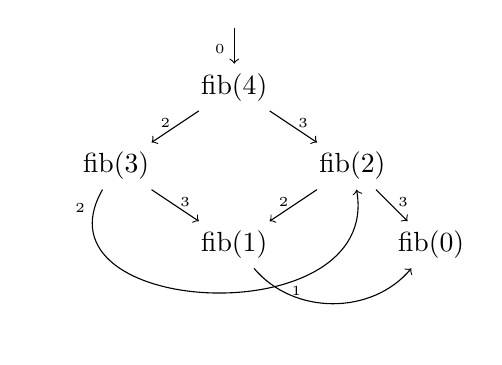
\begin{tikzpicture}
% nodes
\node (f4)     at (2.5, 2) {fib(4)};
    \node (f3) at (1, 1) {fib(3)};
        \node (f1) at (2.5, 0) {fib(1)};
    \node (f2) at (4, 1) {fib(2)};
        \node (f0) at (5, 0) {fib(0)};
% arrows
\draw[<-] (f4) -- node[pos=0.4, left, label distance=5mm]{\tiny{0}} +(0, 0.75);

\draw[->] (f4) -- node[pos=0.4, left, label distance=5mm]{\tiny{2}} (f3);
\draw[->] (f4) -- node[pos=0.4, right, label distance=5mm]{\tiny{3}} (f2);

    \draw[->, bend right=100, out=240, looseness=1.5] (f3) to node[pos=0.05, left, label distance=5mm]{\tiny{2}} (f2);
    \draw[->] (f3) -- node[pos=0.4, right, label distance=5mm]{\tiny{3}} (f1);
    \draw[->] (f2) -- node[pos=0.4, left, label distance=5mm]{\tiny{2}} (f1);
        \draw[->, bend right=50] (f1) to node[pos=0.2, right, label distance=5mm]{\tiny{1}} (f0);
    \draw[->] (f2) -- node[pos=0.4, right, label distance=5mm]{\tiny{3}} (f0);
\end{tikzpicture}
    \subcaption{Callgraph during execution}\label{fig:fib_callstack_graph}
    \end{minipage}%
    \begin{minipage}[b]{.5\linewidth}
    \centering
     
    \begin{tabular}{c|c|c}
        \texttt{in\_1} & \texttt{callsite\_1} & \texttt{out\_1} \\
        \hline
        \hline
        \texttt{NULL} & \texttt{0} & \texttt{4}\\
        \texttt{4} & \texttt{2} & \texttt{3}\\
        \texttt{4} & \texttt{3} & \texttt{2}\\
        \hline
        \hline
        \texttt{3} & \texttt{2} & \texttt{2}\\
        \texttt{3} & \texttt{3} & \texttt{1}\\
        \texttt{2} & \texttt{2} & \texttt{1}\\
        \texttt{2} & \texttt{3} & \texttt{0}\\
        \hline
        \texttt{1} & \texttt{1} & \texttt{0}\\
        \hline
    \end{tabular}
    \subcaption{Tabular representation of the callstack}\label{fig:fib_callstack_table}
    \end{minipage}
    \caption{Callgraph of \texttt{fib(4)} (a) and its tabular representation as generated by the \texttt{callstack}-CTE (b). Each edge represents a callsite.}\label{fig:fib_callstack}
\end{figure}

The callgraph-CTE creates a direct encoding of the actual callstack-tree but collapses identical nodes into one, resulting in a Directed Acyclic Graph (DAG) if the recursion contains no loops (\autoref{fig:fib_callstack}). Each row depicts an edge between two nodes, including the label. Nodes of the callgraph correspond to recursive calls, identified by their arguments, one column per argument. Beside arguments of the caller and callee, the id of the callsite is noted. Callsite ids are used to associate callsites to scenarios.

\subsection{Collecting callsite arguments}

The callgraph is created by an self-referential CTE. The base query and the self-referential query of the CTE are nearly identical. Each callsite has an own query returning a single row (input arguments, callsite id, callsite arguments) if the predicate of its scenario is fulfilled. The template is given in \autoref{marco:collect_call_maybe}.
The predicate acts as guard to add only callsites of the current evaluation scenario. Only if the predicate is fulfilled, any row is returned. For example, the query that returned the third row in \autoref{fig:fib_callstack_table} is generated by \mintinline{postgresql}{<collect_call_maybe(d.out_1, p2, <callsite id: 3, arg_1: (SELECT $1 - 2)>)>}.

\begin{figure}[h!]\centering
    \begin{minted}{postgresql}
    <collect_call_maybe(in_arg_1, predicate, callsite)>
        := SELECT
             in_arg_1                    AS in_1, 
             callsite.id                 AS callsite_id,
             callsite.arg_1[in_arg_1/$1] AS out_1
           FROM predicate AS p(is_true)
           WHERE p.is_true
    \end{minted}
  \caption{Pseudocode to generate a single call to the callgraph-table. $q[y/x]$ denots the operation of replacing $y$ for $x$ in $q$. For \texttt{in\_arg\_1} it is used in the beginning \texttt{\$1} and later references to preceding arguments from the table.}
  \label{marco:collect_call_maybe}
\end{figure}

The macro from \autoref{marco:collect_call_maybe} creates only a query, returning one or none rows. To collect \textit{all} callsites, the query needs to test all callsites of all scenarios (\autoref{macro:collect_calls}). As all callsites within a scenario depend on the same predicate, the scenario-predicate can be pulled up into a CTE to avoid multiple evaluations.

\begin{figure}[h!]\centering\small
    \begin{minted}{postgresql}
    <collect_calls(in_arg_1, scenarios)> :=
        WITH p1 AS (scenarios[1].predicate)[in_arg_1/$1],
             p2 AS (scenarios[2].predicate)[in_arg_1/$1]
             
        -- Scenario 1
        (   -- Callsite 1
            <collect_call_maybe(in_arg_1, p1, scenarios[1].callsites[1])>   )
        
        UNION
        
        -- Scenario 2
        (   -- Callsite 2
            <collect_call_maybe(in_arg_1, p2, scenarios[2].callsites[1])>
          UNION
            -- Callsite 3
            <collect_call_maybe(in_arg_1, p2, scenarios[2].callsites[2])>   )
\end{minted}
  \caption{All callsites of all scenarios needs to be tested to cover the entire UDF.}
  \label{macro:collect_calls}
\end{figure}

With the query generated by \texttt{<collect\_calls(\$1, scenarios)>} all callsites of the initial UDF invocation are obtained. Subsequent levels of the callgraph can be collected recursively by using the \texttt{out\_1}-column from the previous iteration instead of \texttt{\$1}. For each callsite from the previous iteration, the according evaluation scenario needs to be detected to collect new callsites. This for-each behaviour is implemented by \texttt{LATERAL} in the template for \texttt{callgraph}.

\begin{figure}[h!]\centering
\begin{minted}{postgresql}
<callgraph(rec_scenarios)> :=
  (
    (SELECT NULL, 0, $1) -- add original call
      UNION ALL
    <collect_calls($1, rec_scenarios)> 

  ) UNION (
    SELECT
      new_calls.*
    FROM
      callgraph AS c, LATERAL (
        <collect_calls(c.out_1, rec_scenarios)>
      ) AS new_calls
  )
\end{minted}
  \caption{}
  \label{}
\end{figure}


\iffalse
\begin{figure}[h!]
    \centering
    \bgroup
\def\arraystretch{1.5}
\begin{tabular}{|c|}\hline
%\footnotesize\mintinline{postgresql}{in_args := $1 / SELECT c.call_args FROM callstack c}\\
\begin{tabular}{|l|}\hline
    \footnotesize{Scenario 1}\\
    \begin{tabular}{|l|}\hline
        \footnotesize{Callsite 1}\\
        \footnotesize\mintinline{postgresql}{SELECT in_args, callsite.id, callsite.args AS call_args}\\[-5pt]
        \footnotesize\mintinline{postgresql}{  FROM scenario.pred p WHERE p.v}\\
    \hline \end{tabular}\\
    \mintinline{postgresql}{UNION}\\
    \begin{tabular}{|l|}\hline
        \footnotesize{Callsite 2}\\
        \footnotesize\mintinline{postgresql}{SELECT in_args, callsite.id, callsite.args AS call_args}\\[-5pt]
        \footnotesize\mintinline{postgresql}{  FROM scenario.pred p WHERE p.v}\\
    \hline \end{tabular}\\[2mm]
\hline \end{tabular}\\
    \mintinline{postgresql}{UNION}\\
\begin{tabular}{|l|}\hline
    \footnotesize{Scenario 2}\\
    \begin{tabular}{|l|}\hline
        \footnotesize{Callsite 3}\\
        \footnotesize\mintinline{postgresql}{SELECT in_args, callsite.id, callsite.args AS call_args}\\[-5pt]
        \footnotesize\mintinline{postgresql}{  FROM scenario.pred p WHERE p.v}\\
    \hline \end{tabular}\\[2mm]
\hline \end{tabular}
\\[6mm]
\hline
\end{tabular}
\egroup
    \caption{Structure of the callstack CTE. In the beginning, the original parameters \$1 are used. The recursive step iterates over all newly discovered calls.}
    \label{discovery_strucutre}
\end{figure}
\fi

For a complete example of the \texttt{callgraph}-CTE for fib, see \autoref{fib:callstack_cte_complete} in the appendix.

Callgraph growth ends as soon as no recursive scenario is applicable for any newly discovered callsites, ie. all callsites lead to basecases. In this case, the new iteration contains no rows, causing \texttt{WITH RECURSIVE} to stop.

\section{Callgraph evaluation}
% Evaluation starts bottom up at the leaves of the callstack
Evaluation starts bottom up from the leafs of the callgraph. Scenarios are evaluated by replacing their original arguments with references to the arguments from the callgraph (\autoref{macro:single_basecase}). Scenarios may depend on other scenarios that need to be evaluated first. If all dependencies of a scenario are evaluated, the scenario can be evaluated itself. Nonrecursive scenarios have no dependencies and can be therefore evaluated straight ahead. From this initial rows evaluation continues. Finally, the desired result can be selected.

\begin{figure}[h!]\small
    \begin{minipage}[b]{.45\linewidth}\small
    \centering
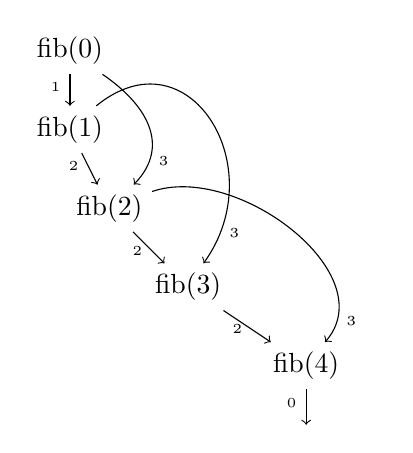
\begin{tikzpicture}
% nodes
\node (n4) at (2.5, -2) {fib(4)};
\node (n3) at (1, -1) {fib(3)};
\node (n2) at (0, 0) {fib(2)};
\node (n1) at (-0.5, 1) {fib(1)};
\node (n0) at (-0.5, 2) {fib(0)};
% arrows
\draw[->] (n0)     to node[pos=0.4,left] {\tiny{1}} (n1);
\draw[->, bend left=40, looseness=1.2, in=120] (n0)     to node[pos=0.8,right] {\tiny{3}} (n2);
\draw[->] (n1)     to node[pos=0.4,left] {\tiny{2}} (n2);
\draw[->, bend left=70, looseness=1.6, out=95] (n1)     to node[pos=0.9,right] {\tiny{3}} (n3);
\draw[->] (n2)     to node[pos=0.6,left] {\tiny{2}} (n3);
\draw[->, bend left=60, looseness=1, in=90] (n2)     to node[pos=0.9,right] {\tiny{3}} (n4);
\draw[->] (n3)     to node[pos=0.6,left] {\tiny{2}} (n4);
\draw[->] (n4)     to node[pos=0.4,left] {\tiny{0}} +(0, -0.75);
\end{tikzpicture}
    \subcaption{}\label{}
    \end{minipage}%
    \hfill
    \begin{minipage}[b]{.45\linewidth}\small
    \centering
    \begin{tabular}{@{}|c|c|@{}}
  \tabname{2}{\strut\texttt{\,evaluation\,}} \\
  \colhd{in\_1} & \colhd{result} \\
  0 & 0 \\
  1 & 1 \\
  2 & 1 \\
  3 & 2 \\
  4 & 3 \\
  \hline
\end{tabular}
    \subcaption{}\label{fig:fib_callstack_cte}
    \end{minipage}
    \caption{a) Dependency-graph, directly retrieved from the callgraph. Callsite ids are annotated to the edges. Sinks are callsites resulting in basecases. b) \texttt{evaluation}-table that holds results for all evaluated scenarios. The first row is the result of the basecase. Following rows are computed iterativly.}\label{}
    \vspace*{-1cm}
\end{figure}

\subsection{Evaluating basecases}
Arguments for the evaluation of nonrecursive scenarios can be found in the leafs of the callgraph.
Evaluation of a single scenario is rather simple. UDF-arguments like \texttt{\$1} are replaced by references to arguments (\texttt{out\_1}) from the callgraph. The predicate from the generated scenario is evaluated in the \texttt{WHERE}-clause and prevents evaluation of wrong scenarios. \autoref{macro:single_basecase} shows a macro for evaluating a single scenario. Each scenario corresponds to a single query returning one or no rows. To collect all scenarios the union of this queries is built.
\begin{figure}[h!]
    \centering
    \begin{minted}{postgresql}
<evaluate nonrecursive scenario(scenario)>
 := SELECT c.out_1                               AS in_1, 
           scenario.query[c.out_1/$1]::<argtype> AS result
    FROM calls_to_basecase c
    WHERE scenario.predicate[c.out_1/$1]
    \end{minted}
    \caption{Macro for nonrecursive scenario evaluation.}
    \label{macro:single_basecase}
\end{figure}

For efficiency, nodes of recursive scenarios are filtered from the callgraph (resulting in CTE \texttt{calls\_to\_basecase}) as they cannot belong to basecases. If a callsite with argument \texttt{out\_1} can be found as input argument \texttt{in\_1} in the callgraph, then \texttt{out\_1} belongs to a recursive scenario. Graphically speaking, the query selects nodes from the callgraph with no outgoing edges (sinks in the callgraph resp. leafs in the calltree), which represents callsites that lead to basecases.

\begin{figure}[h!]
    \centering
    \begin{minted}{postgresql}
<basecases(scenarios)> := 
   WITH calls_to_basecase(out_1) AS (
       SELECT DISTINCT out_1 
       FROM callgraph AS c
       WHERE NOT EXISTS (SELECT NULL FROM callgraph AS c2 WHERE (c2.in_1) = (c.out_1))
   )
   <evaluate scenario(scenario[1], calls_to_basecases)>
     UNION ALL 
   <evaluate scenario(scenario[2], calls_to_basecases)>
    \end{minted}
    \caption{\texttt{basecase}-CTE.}
    \label{macro:basecases}
\end{figure}

The unhandy \texttt{WHERE}-clause could be equivalently written as \mintinline{postgresql}{c.out_1 NOT IN (SELECT c2.in_1 FROM callgraph c2)}. %First, \texttt{IS NOT DISTINCT FROM} is the SQL-way of writing a simple \textit{=} while considering \mintinline{postgresql}{NULL=NULL} as true. This is required since \texttt{NULL} can be an argument of a callsite and needs to be matched with its result-row - tri-state logic hinders that.
The subquery from \texttt{NOT IN} is executed for every row as a subquery while the \texttt{NOT EXISTS}-variant can be executed as a much more efficient anti-join.

\subsection{Recursive scenario evaluation}

The evaluation of recursive scenarios follows the schema of the evaluation of nonrecursive scenarios, but is a bit more involved. Callsite-results must be collected per scenario to decide if the scenario is evaluable yet. Only if all callsites of a scneario are evaluated, the scenario can be evaluated itself.

This operation resembles relational division $\texttt{S} \div \texttt{R}$: When dividing \texttt{S} by \texttt{R}, table \texttt{S} is grouped by the attributes that are not involved as join-attributes with \texttt{R}. The grouped columns from \textit{S} are returned, if every row in the group have found a join-partner from \texttt{S}. By dividing \texttt{callgraph} by \texttt{evaluation} (projecting away \texttt{callgraph.call\_site\_id}), we obtain only those input arguments that are evaluable, ie. have all required callsite-results available.

\begin{figure}[h!]\centering
  \sqlcode{snippets/relational_division.sql}
  \caption{Selecting available callsite-results per scenario using relational division with \texttt{array\_agg}. Does not play well with array-arguments.}
  \label{relational_division}
\end{figure}

The difficulty is to collect those callsite-results. The intuitive approach is to add an \texttt{array\_agg(e.result)} to the relational division (\autoref{relational_division}) that collects the results per scenario. This works well as long as we do not allow arrays as arguments: \texttt{array\_agg} require all input arrays to have the same dimensionality.

The solution is to avoid array aggregation and to "pivot" the groups instead: each callsite-result gets its own column. Pivoting is implemented by using window-functions and partitions together with \texttt{nth\_value} instead of \texttt{GROUP BY} and \texttt{array\_agg}. This way, we circumvent any constraints regarding arrays and avoid expensive aggregation.

With this problem solved, evaluating a recursive scenario boiles down to replacing UDF-arguments and callsites with \texttt{callgraph}- resp. \texttt{evaluation}-references, similar to the evaluation of nonrecursive scenarios (\autoref{macro:single_basecase}). \autoref{macro:recursive_scenario_evaluation} gives a macro to evaluate a scenario utilizing the pivoting approach from above.

\begin{figure}[h!]\small
    \centering
    \begin{minipage}[b]{\linewidth}
    \centering
    \sqlcode{snippets/eval_recursive_scenario.sql}
    \vspace{3mm}
    \subcaption{(b) shows the result of the join, (c) the final result of the generated query and the effects of the ~\WHERE-clauses are annnotated: \circled{1} Do not consider arguments already evaluated callsites. \circled{2} Only consider callsites of the given scenario we are about to evaluate. \circled{3} Only keep rows where all callsites have an result available.}\label{}
    \end{minipage}%
    \caption{Collecting callsite results of for evaluation of a scenario. The result for \texttt{fib(3)} is beeing evaluated. Table (a) shows the result of the }\label{macro:recursive_scenario_evaluation}
\end{figure}
\begin{figure}[h!]
    \ContinuedFloat
    \small
    \centering
    \begin{minipage}[b]{\linewidth}
    \centering
    \begin{tabular}{c|c|p{10cm}p{1em}p{1cm}|c}
      \multicolumn{3}{l}{$\overbrace{\rule{5.2cm}{0pt}}^{\texttt{callgraph}}$}  & ${}^{\bowtie}$ & \multicolumn{2}{l}{$\overbrace{\rule{2.8cm}{0pt}}^{\texttt{evaluation}}$} \\
      \texttt{c.in\_1}                        & \texttt{c.call\_site\_id}  & \multicolumn{3}{c|}{\texttt{c.out\_1 = e.in\_1}} & \texttt{e.res}                                         \\\hline
      \multirow{2}{*}{\color{gray}4}          & \color{gray}2              & \multicolumn{3}{c|}{\color{gray}3}               & \texttt{\color{gray}NULL} \\
                                              & \color{gray}3              & \multicolumn{3}{c|}{\color{gray}2}               & \color{gray}1             \\\hline
      \cellcolor{green!25}                    & \cellcolor{yellow!30}2     & \multicolumn{3}{c|}{2}                           & \cellcolor{blue!20}1             \\
      \cellcolor{green!25}\multirow{-2}{*}{3} & \cellcolor{yellow!30}3     & \multicolumn{3}{c|}{1}                           & \cellcolor{red!20} 1            \\\hline
      \multirow{2}{*}{\color{gray}2}          & \color{gray}2              & \multicolumn{3}{c|}{\color{gray}1}               & \color{gray}1             \\
                                              & \color{gray}3              & \multicolumn{3}{c|}{\color{gray}0}               & \color{gray}0             \\\hline
      \color{gray}1                           & \color{gray}1              & \multicolumn{3}{c|}{\color{gray}0}               & \color{gray}0             \\\hline
    \end{tabular}
    \subcaption{Callgraph table joined with evaluation table.}\label{}
    \end{minipage}%
    \vspace{7mm}
    \begin{minipage}[b]{\linewidth}
    \centering
    \begin{tabular}{rc|c|c|c}
          & \texttt{in\_1} & \texttt{call\_1} \footnotesize{\color{gray}(id: \colorbox{yellow!20}{2})}  & \texttt{call\_2} \footnotesize{\color{gray}(id: \colorbox{yellow!20}{3})} & \texttt{count} \\\cline{2-5}
         \circled{3}                          & \color{gray}\markForTikz{row1Start}{4} & \color{gray}\texttt{NULL}                  & \color{gray}1                     & \color{gray}\markForTikz{row1End}{1} \\\cline{2-5}
         & \cellcolor{green!25}3              & \cellcolor{blue!20}1 & \cellcolor{red!20}1 & 2                                                            \\\cline{2-5}
         \circled{1}                          & \color{gray}\markForTikz{row2Start}{2} & \color{gray}1                              & \color{gray}0                     & \color{gray}\markForTikz{row2End}{2} \\\cline{2-5}
         \circled{2}                          & \color{gray}\markForTikz{row3Start}{1} & \color{gray}1                              & \color{gray}0                     & \color{gray}\markForTikz{row3End}{1} \\\cline{2-5}
    \end{tabular}
    \DrawHLine[thick, opacity=0.5]{row1Start}{row1End}
    \DrawHLine[thick, opacity=0.5]{row2Start}{row2End}
    \DrawHLine[thick, opacity=0.5]{row3Start}{row3End}
    \subcaption{Result of the query. Rows filtered by \WHERE~ are striked through,}\label{}
    \end{minipage}%
    \caption{(continued)}
\end{figure}

The working-table in recursive CTEs contains only the rows from the previous iteration, which is a problem when evaluating. Take the evaluation of \texttt{fib} for example (see \autoref{fig:fib_callstack_graph}): Each recursive scenario depends on the results from the last (\texttt{fib(n-1)}) and the penultimate iteration (\texttt{fib(n-2)}). Standard recursive CTE-semantics allows only access to \texttt{fib(n-1)}.

To work around this restriction, the working table is added to the actual result-rows in each iteration. If we choose this approach, the working-table will be never empty, evaluation would never end. Therefore we need to manually take care of returning the empty table when evaluation should stop. To achieve this, new rows are computed seperately in a CTE and used as guard to prevent addition of the previous results if the CTE contains no rows. \autoref{macro:evaluation_cte}, that shows the final \texttt{evaluation}-CTE, implements this approach.

\begin{figure}[h!]\centering
  \sqlcode{snippets/evaluation_cte.sql}
  \caption{High-level structure of the evaluation-CTE}\label{macro:evaluation_cte}
\end{figure}



\FloatBarrier
\subsection{Result collection and termination}

The previous section introduced the components required to start and continue evaluation of recursive scenarios. The final task is to select the result or to trigger an infinite loop if a setting is detected where the original UDF does not terminate, but the translation has.

There are two ways how a recursive function may not terminate: Infinite recursion and looping calls. Infinite recursion leads always to new calls, never reaching a basecase, the callgraph is infinite. Each new call results in a new, different row that is added to the callgraph-table (\autoref{fig:infinite_callstack}). In this case, the translation does not terminate correctly, as the original.

\begin{figure}[h!]\small
    \begin{minipage}[b]{.5\linewidth}
    \centering
    \begin{minted}{sql}
SELECT CASE WHEN n = 0 THEN 0
            ELSE f(n-2)
       END
    \end{minted}
    \subcaption{UDF-body of a function \texttt{f}}
    \label{fig:infinite_callstack_udf}\par\vfill
    \end{minipage}%
    \begin{minipage}[b]{.5\linewidth}
    \centering
    \begin{tabular}{c|c|c}
in\_n & callsite & param\_n \\\hline
3  & 1 &  1 \\
1  & 1 & -1 \\
-1 & 1 & -3 \\
-3 & 1 & -5 \\
$\vdots$ & $\vdots$ & $\vdots$
    \end{tabular}
    \subcaption{Callgraph of that function. Recursion without a basecase.}
    \label{fig:infinite_callstack_callstack}
    \end{minipage}
    \caption{The function misses its basecase if called with an odd number like 3 and does not terminate. Every call leads to a new, different recursive call as call-arguments grow towards infinity.}\label{fig:infinite_callstack}
\end{figure}

The other case is looping calls. Since we utilize memoization, redundant calls lead only to a single row in the callgraph-table and not to multiple identical rows. Thus, the callgraph-table is finite while the original callgraph is not. Therefore, our implementation would terminate while the original does not. To maintain the original UDf behaviour we need to detect this case and trigger an infinite loop manually.

\begin{figure}[h!]\small
    \begin{minipage}[b]{.45\linewidth}
    \centering
    \begin{minted}{sql}
SELECT CASE WHEN n = 0 THEN 0
            WHEN n = 2 THEN f(0)
            ELSE f(n % 2) + f(2)
       END
    \end{minted}
    \subcaption{}\label{fig:some_loop_udf}
    \end{minipage}%
    \begin{minipage}[b]{.3\linewidth}
    \centering
    \begin{tabular}{c|c|c}
in\_n & callsite & param\_n \\\hline
3 & 2 & 1 \\
3 & 3 & 2 \\
2 & 1 & 0 \\
1 & 2 & 1 \\
1 & 3 & 2
    \end{tabular}
    \subcaption{}\label{fig:some_loop_callstack}
    \end{minipage}
    \begin{minipage}[b]{.2\linewidth}
    \centering
    \begin{tabular}{c|c}
in\_n & result \\\hline
0 & 0 \\\hline
2 & 0 \\
    \end{tabular}
    \subcaption{}\label{fig:some_loop_evaluation}
    \end{minipage}
    \caption{a) UDF-body of a function \texttt{f} where only some part of the callstack causes a loop. b) The callstack is finit, due to memoization. c) Evaluation can start, because some basecases are present, but has not all results available to finish evaluation up to the original call-arguments \texttt{3}.}\label{fig:some_loop}
\end{figure}

How is this situation detectable? If at least one path in the callgraph contains a loop, this path have no basecase where evaluation could start and thus evaluation will stop eventually without having evaluated the root-node. There is no row in the \textit{evaluation}-CTE containing a result for the original UDF-arguments. Instead of returning an empty table, an infinite loop is triggered (\autoref{fig:some_loop}).

\begin{figure}[h!]
    \centering
    \sqlcode{snippets/result_collection.sql}
    \caption{Result collection}
    \label{macro:result_collection}
    \vspace*{-3cm}
\end{figure}


\chapter{Analysis rules}\label{chapter:analysis}

% Intuition how scenario analysis works, then formal inference rules are presented
% Begin with four rules to translate the core of each recurisve UDF
% Extending scope to whole queries
% Adding CTEs
% Post processing

This chapter gives detailed insights of how a given query is sliced into its scenarios and predicates by presenting inference rules. Before each inference rule, I give an intuition of the idea first, before formalizing it.

I begin with presenting a set of four rules that are required to translate most basic \CASE-expressions. The nonrecursive rules \RREC und \RBASE handle the base cases when the SQL-fragment is directly a recursive call resp. does not contain any call at all. Disassembling \CASE-expressions is the true core of the translation process as it is the origin of any scenario. Each \WHEN-\THEN~branch is processed step by step by the \RWHEN-rule and eventually the \ELSE-branch by the \RELSE-rule.

To translate expressions and whole queries four further rules are required that all boil down to a common idea. This idea is that functions have a number of recursive operands that can be translated independently from each other. The different combinations of argument-scenarios form different scenarios of the function itself. Functions in this context can not only be actual functions like \texttt{+}, \texttt{GREATEST} or \texttt{fib}), but also any syntactic construct (eg. \texttt{IS BETWEEN}, \texttt{INNER JOIN}, \texttt{UNION}) that can be understood as one computation step with independent arguments. This schema is also applicable for select- and from-clauses.

Finally, we allow the use of CTEs that come with a couple of complexities. Due to CTEs, it is possible that a recursive SQL-fragment does not contain a callsite directly but indirect via referenced CTEs. Furthermore, CTEs can reference other CTEs so it is necessary to track CTE-dependencies and maintain a list of recursive CTEs while taking shadowing into account.

To retrieve the intermediate representation used by the templates, each scenario is augmented with additional information. Most notably, callsite-arguments are extracted from the surrounding query. I provide a set of inference rules that perform this task while handling CTE the same way as in the rules for scenario generation.

\section{Preliminaries}\label{approach}

\subsection{Structural Operational Semantics}

A Structural Operational Semantic is an abstract way to define program evaluation step by step. Formally stated, it defines relations between states of an abstract machine. A state $S = (E, c)$ consists of an environment $E$ and some "code" $c$. Relations define transitions between two states. The notation $S \rightarrow S'$ (read: "$S$ evaluates \textit{in one step} to $S'$") is so just a shorthand for $(S, S') \in \rightarrow$ where $\rightarrow$ is the relation. In my rules, the environment does not change during a rule application so we can shorten notation and write $E \vdash c \rightarrow c'$. \cite[Chapter 2]{semanticsWithApplications}

A rule may have a number of \textit{premises} $p_1, p_2, \dots, p_n$ that must hold for the rule to be applicable. This premises are written on top of a line above the rule. This premises may include \textit{judgments} over transitions $T \rightarrow^* T'$, that depict that two states are element of the reflexive transitive closure of the relation, ie. that $T$ can be evaluated to $T'$.

$$\quad(\textsc{name})\inferrule{
   p_1\\
   p_2\\
   \dots\\
   p_n
}{
    S \rightarrow S'
}$$

Evaluation happens by recursively applying transition rules from a starting state. Premises that include judgments causes a callstack to build up until an axiom returns eventually a result (right part of the arrow). In the context of analyzing queries, many premises analyze a part of the query and than wraps the result into its own structure.

The provided rules give deterministic evaluation steps, ie. at most one rule is applicable at a time. This makes the rules a bit more verbose, but simplifies implementation as no backtracking need to be implemented to find the applicable rule.

In the case of the scenario analysis, the state is $(C, T, q, r)$. $C$ is a ordered set of tuples. $C[\{a, b\}]$ returns a subset of $C$ with elements with an alias of $a$ or $b$. The empty CTE-store is denoted as $\varnothing$. $T$ is a set of aliases of CTEs. $q$ is the input query and $r$ is the result of the analysis. $C$ and $T$ are taken as environment.

The analysis result $r$ is a tuple $(B, R)$ containing a set of nonrecursive (basecase) scenarios in $B$ and a set of recursive scenarios in $R$. Each scenario consists of a predicate $p$ and a query that represents a "slice" of the original UDF $q$. An analyzsis result with three scenarios could like this:
$$
\Big(
    \overbrace{\big\{
        \underbrace{
            (p_1, q_1)
        }_{\text{scenario 1}}
    \big\}}^{\text{basecase scenarios}}
    ,
    \overbrace{\big\{
        \underbrace{
            (p_2, q_2)
        }_{\text{scenario 2}},
        \underbrace{
            (p_3, q_3)
        }_{\text{scenario 3}}
    \big\}}^{\text{recursive scenarios}}
\Big)
$$

\subsection{Subset of SQL}
Rules to analyze arbitrary queries would need to consider every single language construct. Instead, we focus on a smaller subset of SQL (\autoref{lst:sql_grammar}) to keep the number of rules small and demonstrate the core idea. Generalizations can be added later, if necessary. The grammar describes nested \texttt{SELECT-FROM-WHERE} queries (S-F-W) with (nonrecursive) CTEs and query-combining functions.

Functions in the grammar are stated in praefix-notation, even if the actual function comes in the form of eg. \texttt{i IS BETWEEN a AND b}, \texttt{x[n]} or \texttt{a IN (<query>)}. Those syntactic details are not visible when represented as AST and all constructs that act like a function are considered a function during translation.

\begin{figure}[H]
    \begin{minted}{postgresql}
    <query>     ::= [ WITH (<query>) AS <tblAlias>[, ...] ]
                      SELECT <expr>  AS <colAlias>[, ...]
                    [ FROM <tbl>     AS <tblAlias>[, ...] ]
                    [ WHERE <expr> ]
                 |  <query> { UNION | INTERSECT | EXCEPT } [ALL] <query>
    <tbl>       ::= <tblRef> | (<query>) | <fun>([<expr>, ...])
    <expr>      ::=  <const> |  <colRef> |  <fun>([<expr>, ...])
                 |  CASE [WHEN <expr> THEN <expr>, ...] ELSE <expr> END
                 |  ( <query> )
    <fun>       ::= Stable functions
    <const>     ::= SQL built-in constants
    <tblAlias>  ::= alias(colAlias[, ...])
    <colAlias>  ::= alias
    \end{minted}
    \caption{The subset of SQL that is targeted by the inference rules.}
    \label{lst:sql_grammar}
\end{figure}


%\subsection{No VOLATILE functions}
%Without referential transparancy we cannot assume that two function calls within the same query return the same value, making it impossible to use memoization. Therefore, only UDFs markes as STABLE or IMMUTEABLE (38.7. Function Volatility Categories) are translateable.

\subsection{Notation and vocabulary}

We say a query-fragment $q$ of an UDF named $fn$ contains a callsite or is recursive, if the AST of $q$ contains a node with a call to the $fn$ itself or references a recursive table-variable. The latter is a bit involved (see \autoref{tracking_recursive_ctes}), so we use a simplified variant of $\hasCallsite$ for the beginning that does not take references into account:

$$\hasCallsite(e) = fn \sqsubset e$$

%The auxiliary function $\sigma_{\text{cols}}$ is used to pick columns from the store by name, eg. $\sigma_{a, t, p, r}(C)$ returns the entire store $\langle (a, t, p, r)_1, \dots, (a, t, p, r)_n \rangle$ and $\sigma_p(C) = \langle p_1, \dots, p_n \rangle$ all predicates in the store.


% UDF is analyzed and a intermediate representation is created that is used as input for the query template. 
% Each scenario consists of a single path through the case-distinctions of the original query. A predicate is generated alongside to detect when this path is taken. Recursive and nonrecursive scenarios are distinguished.
% Scenarios are generated by recursively applying inference rules to the original function-body. The idea behind each rules is first illustrated before the formal definition is presented
% I will begin with four rules necessary to translate the heart of every recurisve UDF, the CASE-expression. Then I will extend the scope to cover arbitrary "function-alikes" from `+` to whole queries. I complete with rules to handle CTEs, which will introduce a couple of complexities that need special considerations.
% Before the scenarios can be used to fill in the query template, some postprocessing is needed. Callsites need to be enumerated and scenarios must be augmented with a list of contained scenarios. Furthermore, arguments must be extracted to individual queries.

%There are two base-rules that require no more rule application and lead to an immidiate result: \RBASE and \RREC. The \RBASE-rule is applicable when a subtree $q$ contains no recursive calls or references to recursive table-expressions. We directly obtain the resulting tuple $(\{q\}, \emptyset)$. The other case is the \RREC-rule, which handles a subtree $q$ where the root node is the recursive call itself. To comply with the overall restrictions given under X.Y.Z, no argument may have a callsite. If this is given, the rule leads directly to $(\emptyset, \{q\})$. TODO: EXPLAN REF

%All other rules require a callsite somewhere within the query, unwrapping each layer of the query until the callsite is reached or no callsite exists in the subtree. The rules for handling \CASE-statements create for each possible outcome one pruned version while extending the given predicate by the predicate of the taken \WHEN-branch. In contrast to SELECT-statements and CASE-expressions, other parts of the query \textit{can} contain callsites in sibling subtrees. The idea here is to compute all possible outcomes of these subtrees independantly and then build the cartesian-product to receive all possible scenarios of the execution of the parent node. The \REXPR-rule implements purely this idea and the \RCTE and \RFROM-rule come as variations or extensions that take distinct particularities into account.

%The most complicated rule is for handling \WITH-statements. As in the \REXPR-rule, each execution-scenario for every CTE is computed and then the cartesion-product is build over all the scanarios. But two difficulties needs to be considered: First, each CTE can reference previous CTEs from within the same WITH-statement. Second, not every CTE may be referenced later on when the actually query (without the CTEs) is processed - eg. the referencing part may be pruned away after application of a \RWHEN-rule. This leads to to multiple identical versions of the original query that only differ in their predicates, namely by the case-distinctions from the unused CTE. This is semantically not a problem but can degrade performance, since callsites are enumerated based on the set of recursive and nonrecursive cases. Unfortunately, it is hardly possible to postpone this step to postprocessing since we would have to identify and remove the parts caused by the unused CTE from the predicate. Thus we hve two rules for handling CTEs: One for processing and removing each CTE one by one from the query and one for reconstructing the original \WITH-Statement, limited to that CTEs that are actually used by the translated query eventually.

%So, how does the CTE-Rules work in detail? Each CTE is processed on its own, one by one. The processed CTE is removed from the query and put into the variable-store and added alongside with its predicate to the temporary CTE-list. Depending on the processed CTE the recursive or nonrecursive store/list is choosen. Computation continues as long as CTEs are present. Finally, the complete query including CTEs is reconstructed. The actual query is translated with emptied temporary CTE-lists. Only CTEs that are referenced (directly or indirectly) are kept and their predicates are appended to the result predicate. To find out what CTEs are referenced, all free variables under the given environment need to be recursivly followed.

\section{Translating simple \texttt{CASE}-expressions}
% Goal is to translate a simple CASE-statement
% Start with primitive rules that do not recurse
% Within CASE-expressions the callsite can be located at two different places: WHEN and THEN
% CASE-expressions can be nested, again this can happen in the WHEN and in the THEN part.

For this section, we focus on the rules that are involved in every translation. First, those are two axioms that will eventually add an expression either to $B$ or to $R$. Secondly, those are rules for handling \texttt{CASE}-expressions. I will illustrate the different possible situations that need to be considered when processing a \texttt{CASE}-expressions, before formalizing the \RWHEN-rule. With those four rules it is already possible to analyze very simple expressions.

\subsection{Callsites and basecases}

The leafs of every derivation tree are axioms. The two most important axioms are \RREC and \RBASE (see \autoref{rule:base_and_rec}). They assign an query-fragment either to the set of recursive ($R$) or non-recursive scenarios ($B$). The distinction is made by the presence of a \textit{callsite} in the given query-fragment. The predicate $\hasCallsite(T, e)$\footnote{Please ignore the argument $T$ of $\hasCallsite$ and the environment $T, C$ of the rules for now, we will come back to this later.} returns true if an actual recursive call to $fn$ is located in the subtree of the AST-representation of the query-fragment $e$.

%The inference rules are applied recursively to an initial query, processing each layer one by one. In the end, each derivation treeare two axioms\footnote{By definition, an axiom has no premises. Premises without further rule application are actually side-constraints that limit rule applicability. Therefore this rules are considered anyway "axioms".}. Either we arrive at a \textit{callsite}, ie. the invocation of the recursive function itself, or the current subtree contains no callsite at all. In the latter case, it is not necessary to descend any further, we can consider the remaining subtree as basecase.

\begin{figure}[h]\small
    \begin{minipage}[b]{\linewidth}
    \centering % BASE
    
  $$
\quad(\textsc{base})\inferrule{
   \neg \hasCallsite(T, e) \\
   \neg \text{isElse}(e)
}{
    T, \varnothing \vdash (p, e) \rightarrow (\{(p, e)\},\{\})
}$$
    \subcaption{}\label{rule:base}
    \end{minipage}\\
    \begin{minipage}[b]{\linewidth}
    \centering % REC
$$\quad(\textsc{rec})\inferrule{
   \forall i \in \{1, ..., n\} : \neg \hasCallsite(T, x_i)
}{
    T, C \vdash (p, fn(x_1, ..., x_n)) \rightarrow (\{\}, \{(p, fn(x_1, ..., x_n))\})
}
$$
    \subcaption{}\label{rule:rec}
    \end{minipage}
    \caption{Rule (a) assigns any query-fragment to $B$ if it does not contain any callsites. (b) Does handle callsites by adding them to $R$. For now, please ignore $T$ and $C$.}\label{rule:base_and_rec}
\end{figure}

The \RREC-rule enforces that no callsite may have a recursive argument. This restriction is due to the strategy how we build the callgraph. It is based on evaluating the arguments of the callsites independently from the whole query. If the arguments itself would be recursive, this is not possible.

\subsection{Simple \CASE-expressions}
\begin{wrapfigure}{r}{.3\textwidth}\centering
\begin{minted}{postgresql}
CASE WHEN p1 THEN r1
     WHEN p2 THEN r2
     ELSE         r3
END
\end{minted}
\caption{A simple \texttt{CASE}-expression}\vspace{-5mm} 
\label{lst:case}
\end{wrapfigure}

The other rules that are endeavoured in every nontrivial translation are those for handling \texttt{CASE}-expressions (\autoref{lst:case}). They are the original source of any scenario generated. \texttt{CASE}-expressions are \textit{conditional-expression}, other conditionals are \texttt{COALESCE}, \texttt{NULLIF}, \texttt{GREATEST} and \texttt{LEAST}. All of them can be rewritten as \texttt{CASE} (see \autoref{sql:conditionals}).

\texttt{CASE}-expressions in general are a handy way of writing nested \texttt{IF}s. Each \texttt{WHEN} implies that all preceding \texttt{WHEN}'s have failed, ie. each \texttt{WHEN} contains an implicit negation of all preceding \texttt{WHEN}'s. Our goal is to make the implicit complete predicate explicit so that it can be executed independently.

\autoref{flow:simple_case} visualizes the logical flow of a simple \texttt{CASE}-expression with callsites located in the first \texttt{WHEN} and in the \texttt{ELSE}-branch. An arrow to the right means that the predicate is fulfilled, an arrow down denotes the negation. Predicates $p_i$ are surrounded by a single lined border while doubled bordered box marks a possible result $r$ of the \texttt{CASE}-statement. An asterisk $\ast$ indicates a query-fragment that includes a recursive subexpressions (according to $\hasCallsite$).

The segmented rectangles at the right (\autoref{scenarios:simple_case}) depict the generated scenarios from the \texttt{CASE}-expression. The asterisk flags a scenario as recursive ie. $\in R$, otherwise $\in B$. The second segment contains the predicate of the scenario, followed by the query, the actual slice of the original UDF.

\begin{figure}[h!]
    \begin{minipage}[b]{.45\linewidth}
    \centering
    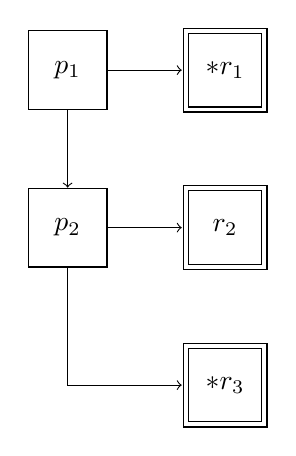
\begin{tikzpicture}[x=20mm, y=20mm]
        \tikzset{Pred/.style={shape=rectangle, draw, minimum width=1cm, minimum height=1cm}}
        \tikzset{Res/.style={shape=rectangle, draw, double distance=0.5mm, outer sep=0.5mm, minimum width=1cm, minimum height=1cm}}
        
        % nodes
        \node[Pred] (p1) at (0, 2) {$p_1$};
        \node[Res]  (r1) at (1, 2) {$\ast r_1$};
        
        \node[Pred] (p2) at (0, 1) {$p_2$};
        \node[Res] (r2) at (1, 1) {$r_2$};
        
        \node[Res] (r3) at (1, 0) {$\ast r_3$};
        
        % arrows
        \draw[->] (p1) -> (r1);
        \draw[->] (p1) -- (p2);
        \draw[->] (p2) -- (r2);
        \draw[->] (p2) |- (r3);
    \end{tikzpicture}
    \subcaption{Logical flow of a simple \CASE-expression with callsites in $r_1$ and $r_3$.}\label{flow:simple_case}
    \end{minipage}\hfill
    \begin{minipage}[b]{.45\linewidth}
    \centering 
    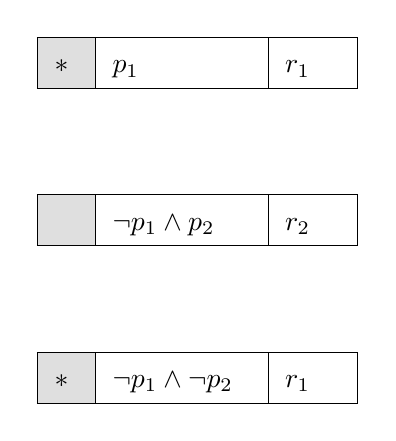
\begin{tikzpicture}[x=20mm, y=20mm]
        \node (case1) at (5, 2) {\begin{tabular}{|p{3mm}|p{5em}|p{2em}|}\hline
        \cellcolor{gray!25} $\ast$ & $p_1$ & $r_1$\\\hline
        \end{tabular}};
        
        \node (case1) at (5, 1) {\begin{tabular}{|p{3mm}|p{5em}|p{2em}|}\hline
        \cellcolor{gray!25} ~~ & $\neg p_1 \land p_2$ & $r_2$\\\hline
        \end{tabular}};
        
        \node (case1) at (5, 0) {\begin{tabular}{|p{3mm}|p{5em}|p{2em}|}\hline
        \cellcolor{gray!25} $\ast$ & $\neg p_1 \land \neg p_2$ & $r_1$\\\hline
        \end{tabular}};
    \end{tikzpicture}
    \subcaption{Generated scenarios for each branch of the \CASE-expression.}\label{scenarios:simple_case}
    \end{minipage}
    \caption{}\label{rule:base_and_rec}
\end{figure}

%\setlength{\tabcolsep}{2pt}

\subsection{Recursive \WHEN's}

Recursive predicates cannot be evaluated during callgraph creation and are therefore considered as part of the result (recursive) expression. Slicing stops \textit{before} the recursive predicate and the entire remaining \texttt{CASE}-expression is considered a single big recursive scenario.

\begin{figure}[h!]
    \centering
\begin{tikzpicture}[x=20mm, y=20mm]
\tikzset{Pred/.style={shape=rectangle, draw, minimum width=1cm, minimum height=1cm}}
\tikzset{Res/.style={shape=rectangle, draw, double distance=0.5mm, outer sep=0.5mm, minimum width=1cm, minimum height=1cm}}

% nodes
\node[Pred] (p1) at (0, 1.5) {$p_1$};
\node[Res]  (r1) at (1, 1.5) {$r_1$};
\node at (4, 1.5) {\begin{tabular}{|p{3mm}|p{5em}|p{2em}|}\hline
\cellcolor{gray!25} & $p_1$ & $r_1$\\\hline
\end{tabular}};

\node[Res, inner sep=3mm] (res) at (0.5, 0) {
    \begin{tikzpicture}[x=20mm, y=20mm, inner sep=1em]
        \node (p2) at (0, 1) {$\ast p_2$};
        \node (r2) at (1, 1) {$r_2$};
        \node (r3) at (1, 0) {$r_3$};
        \draw[->] (p2) -- (r2);
        \draw[->] (p2) |- (r3);
    \end{tikzpicture}
};
\node at (4, 0) {\begin{tabular}{|c|c|c|}\hline
\cellcolor{gray!25} $\ast$ & $\neg p_1$ & $\CASE ~ \WHEN ~p_2~ \THEN ~r_2~ \ELSE ~r_3~\END$\\\hline
\end{tabular}};
% arrows
\draw[->] (p1) -> (r1);
\draw[->] (p1) -> (0, 0.95);
\end{tikzpicture}
    \caption{Logical flow and resulting scenarios of a \texttt{CASE}-expression with a recursive predicate. Everything after and including the recursive predicate is considered one single recursive scenario.}
    \label{fig:my_label}
\end{figure}

This introduces a important overall constraint: No more callsites after a recursive predicate. The template for the callgraph creation makes the assumption that all callsites in a scenario will be evaluated. If the evaluation of one callsite is actually conditioned by the evaluation of an other, our translation evaluates both if they occur in the same scenario. This would cause runtime errors or nontermination.

\subsection{Nonrecursive subtrees}
Subtrees with no callsite are taken as one big basecase. There is no need to do any further analysis because there are no more callsites that need to be seperated into their evaluation scenarios so that the callgraph can be built. In this case, the \RBASE-rule just adds the entire remaining \texttt{CASE}-expression to $B$.

\begin{figure}[h!]
    \centering
\begin{tikzpicture}[x=20mm, y=20mm]
\tikzset{Pred/.style={shape=rectangle, draw, minimum width=1cm, minimum height=1cm}}
\tikzset{Res/.style={shape=rectangle, draw, double distance=0.5mm, outer sep=0.5mm, minimum width=1cm, minimum height=1cm}}

% nodes
\node[Pred] (p1) at (0, 1.5) {$p_1$};
\node[Res]  (r1) at (1, 1.5) {$\ast r_1$};
\node at (4, 1.5) {\begin{tabular}{|p{3mm}|p{5em}|p{2em}|}\hline
\cellcolor{gray!25} $\ast$ & $p_1$ & $r_1$\\\hline
\end{tabular}};

\node[Res, inner sep=3mm] (res) at (0.5, 0) {
    \begin{tikzpicture}[x=20mm, y=20mm, inner sep=1em]
        \node (p2) at (0, 1) {$p_2$};
        \node (r2) at (1, 1) {$r_2$};
        \node (r3) at (1, 0) {$r_3$};
        \draw[->] (p2) -- (r2);
        \draw[->] (p2) |- (r3);
    \end{tikzpicture}
};
\node at (4, 0) {\begin{tabular}{|c|c|c|}\hline
\cellcolor{gray!25} ~~ & $\neg p_1$ & $\CASE ~ \WHEN ~p_2~ \THEN ~r_2~ \ELSE ~r_3~\END$\\\hline
\end{tabular}};
% arrows
\draw[->] (p1) -> (r1);
\draw[->] (p1) -> (0, 0.95);
\end{tikzpicture}
    \caption{A \texttt{CASE}-expression where no of the later branches have a callsite. Therefore the \RBASE-rule takes them all as a basecase.}
    \label{fig:case_nonrecursive}
\end{figure}


\subsection{Nested \texttt{CASE}-expressions}

\texttt{CASE}-expression can be nested. Nesting can happen either within the predicate of the \texttt{WHEN}-part, or within the result of \texttt{THEN}-part. As dependant callsites are forbidden, either the predicate or the result can have a nested \texttt{CASE}-expression with a callsite, but not both. If there is a nested \texttt{CASE}-expression without a callsite, it is left unchanged (\RBASE-rule).

If a \CASE-expression is located in the \texttt{THEN}-part, the inner expression is analyzed independently. The predicate from the outer scenario is prepended to the predicates of the scenarios that are generated by the inner \CASE-expression.

%Predicates must be evaluable directly for our translation template, ie. no callsite may be present in any predicate. Therefore, as soon as a predicate appears to be recursive, the recursive predicate is considered part of the recursive result and the evaluation of the \CASE-expression halts with the remaining \CASE-expression which forms an recursive case as a whole.
\begin{figure}[h!]
    \centering
    \begin{tikzpicture}[x=20mm, y=20mm]
\tikzset{Pred/.style={shape=rectangle, draw, minimum width=1cm, minimum height=1cm}}
\tikzset{Box/.style={shape=rectangle, draw, minimum width=1cm, minimum height=1cm, dotted, very thick}}
\tikzset{Res/.style={shape=rectangle, draw, double distance=0.5mm, outer sep=0.5mm, minimum width=1cm, minimum height=1cm}}

% nodes
\node[Pred] (p) at (0.5, 1) {$p$};
\node[Box]  (r1) at (2, 1) {
    \begin{tikzpicture}[x=15mm, y=15mm]
        \node[Pred] (p1) at (0, 2) {$p_1$};
        \node[Res] (r1) at (1, 2) {$r_1$};
        
        \node[Pred] (pi) at (0, 1) {$p_2$};
        \node[Res] (ri) at (1, 1) {$r_2$};
        
        \node[Res] (rn) at (1, 0) {$\ast r_3$};
        % arrows
        \draw[->] (p1) -- (r1);
        \draw[->] (pi) -- (ri);
        \draw[->] (p1) -- (pi);
        \draw[->] (pi) |- (rn);
    \end{tikzpicture}
};
\node at (5, 1.75) {
    \begin{tabular}{|p{1em}|p{2.5cm}|c|}\hline
    \cellcolor{gray!25}  & $p \land \phantom{\neg}p_1$ & $r_1$\\\hline
    \end{tabular}
};
    
\node at (5, 1) {
    \begin{tabular}{|p{1em}|p{2.5cm}|c|}\hline
    \cellcolor{gray!25}  & $p \land \neg p_1 \land \phantom{\neg} p_2$ & $r_2$\\\hline
    \end{tabular}
};

\node at (5, 0.25) {
    \begin{tabular}{|p{1em}|p{2.5cm}|c|}\hline
    \cellcolor{gray!25}$\ast$   & $p \land \neg p_1 \land \neg p_2$ & $r_3$\\\hline
    \end{tabular}
};
   
% arrows
\draw[->] (p) -- (r1);
\end{tikzpicture}
    \caption{Nested \texttt{CASE} in the predicate.}
    \label{fig:case_nested_in_when}
\end{figure}

If a recursive \texttt{CASE}-expression is nested inside the \texttt{THEN}-part, it is analyzed and number of scenarios is returned. The particularity here is that the results of the scenarios are predicates. Thus, the scenario of the nested \texttt{CASE}-expression contains a predicate and a predicate for the predicate. Therefore both, the predicate and the result of the inner scenario, need to be added to the predicate of the scenario of the outer \texttt{CASE}-expression.

\begin{figure}[h!]
    \centering
\begin{tikzpicture}[x=15mm, y=12mm]
\tikzset{Pred/.style={shape=rectangle, draw, minimum width=1cm, minimum height=1cm}}
\tikzset{Box/.style={shape=rectangle, draw, minimum width=1cm, minimum height=1cm, dotted, very thick}}
\tikzset{Res/.style={shape=rectangle, draw, double distance=0.5mm, outer sep=0.5mm, minimum width=1cm, minimum height=1cm}}

% dash pattern=on 5pt off 1pt on 3pt off 3pt on 1pt off 2pt on 1pt off 2pt on 3pt off 1pt

% nodes
\node[Pred] (p) at (0, 3) {$p$};

\node[Box] (p1) at (0, 1) {
    \begin{tikzpicture}[x=15mm, y=15mm]
        \node[Pred] (p2) at (0, 1) {$\pi_1$};
        \node[Pred] (r2) at (1, 1) {$p_1$};
        \node[Pred] (p3) at (1, 0) {$\ast p_2$};
        % arrows
        \draw[->] (p2) -- (r2);
        \draw[->] (p2) |- (p3);
    \end{tikzpicture}
};
\node[Res] (r1) at (2, 1) {$r_i$};
\node (case1) at (6, 1) {
    \begin{tabular}{|p{1em}|r|c|}\hline
    \cellcolor{gray!25} & $\neg p \land \pi_1 \land \phantom{\neg} p_1$ & $r_i$\\\hline
    \cellcolor{gray!25} & $\neg p \land \pi_1 \land \neg p_1$ & $r$\\\hline
    \end{tabular}
};

\node[Res] (r) at (2, -1) {$r$};
\node (case1) at (6, -1) {
    \begin{tabular}{|p{1em}|r|c|}\hline
    \cellcolor{gray!25} $\ast$ & $\neg p \land \neg \pi_i$ & \texttt{WHEN }$p_2$ \texttt{THEN} $r_i$ \texttt{ELSE} $r$\\\hline
    \end{tabular}
};
% arrows
\draw[->] (p) -- (p1);
\draw[->] (p1) -- (r1);
\draw[->] (p1) |- (r);
\end{tikzpicture}
    \caption{Nested \texttt{CASE} in \texttt{WHEN}-part. Note that neither $r_i$ nor $r$ must contain any callsite.}
    \label{fig:case_nested_when}
\end{figure}

\subsection{\CASE- and \ELSE-rule}

The \RWHEN-rule works branch by branch. It is only applicable if not both, the predicate $p$ and the remaining branches $bs$, contain callsites (1st premise). Predicate $p$ and resulting expression $e$ are analyzed, obtaining scenarios $(B_p, R_p)$ for the predicate and $(B_e, R_e)$ for the resulting expression (2nd and 3rd premise). The nonrecursive scenarios of the predicate $B_p$ contain $n$ tuples of a predicate (of the scenario, ie. the "predicate of the predicate") and a result, the actual predicate (4th premise).

The last premise analyzes the remaining branches for those scenarios where the predicate is nonrecursive (from $B_p$). The predicate of the remaining branches is thus prepended with the (positive) predicate of the predicate $p_p$ and the negated actual predicate $p'$. The scenarios from later branches are added in the actual rule to set of non-/recursive scenarios.

\begin{figure}[h!]
    \centering\small

  \makebox[\textwidth][c]{$$\inferrule{
    \neg (\hasCallsite(T, p) \land \hasCallsite(T, bs))\\\\
    T, C \vdash (\TRUE, p) \rightarrow (B_p, R_p) \\\\
    T, C \vdash (\TRUE, e) \rightarrow (B_e, R_e)\\\\
    B_p = \{(p_{p_1}, p'_1), ..., (p_{p_n}, p'_n)\} \\\\
    \forall 1 \leq i \leq n : T, C \vdash (p_0 ~\AND~ p_{p_i}~\AND~\NOT~ p'_i,~ \CASE~ bs ~\END) \rightarrow (B_i, R_i) \\
}{
T, C \vdash (p_0, \CASE~ \WHEN ~p ~\THEN ~e ~bs ~\END) \rightarrow \\
{\begin{tabular}{L}
         \Big( \Big\{\big(p_0 ~\AND~ p_p         ~\AND~ p' ~\AND~ p_e , e'\phantom{\CASE ~ \WHEN ~  ~ \THEN ~e ~bs~ \END}\big) ~|~~(p_p, p') \in B_p, (p_e, e') \in B_e \Big\} \cup~ (\cup_{1\leq i \leq n}B_i)~~~~,\\[2mm]
\phantom{\Big(}\Big\{\big(p_0 ~\AND~ p_p         ~\AND~ p' ~\AND~ p_e , e'\phantom{\CASE ~ \WHEN ~  ~ \THEN ~e ~bs ~\END}\big) ~|~~(p_p, p') \in B_p, (p_e, e') \in R_e \Big\} \cup~ (\cup_{1\leq i \leq n}R_i) ~\cup\\
\phantom{\Big(}\Big\{\big(p_0 ~\AND~ p_p\phantom{~\AND~ p' ~\AND~ p_e},            \CASE ~ \WHEN ~p'~ \THEN ~e ~bs ~\END \big) ~|~~(p_p, p') \in R_p~~~~~~~~~~~~~~~~~  \Big\}~~~~~~~~~~~~~~~~~~~~~~~~~ \Big)
\end{tabular}}
}\quad(\textsc{when})$$}
    \caption{\RWHEN-rule to slice \texttt{CASE}-expressions into its different evaluation scenarios.}
    \label{fig:my_label}
\end{figure}

The actual rule combines all sources of scenarios. The basecase scenarios (first component of the tuple) are built by combining all nonrecursive predicates ($B_p$) with the nonrecursive resulting expressions ($B_e$). These set of scenarios is unioned with the $n$ sets of scenarios from other branches $(B_i, R_i)$ (remember that $n$ is the number of nonrecursive predicate-scenarios).

The same happens analogiously for the second component of the tuple, the recursive scenarios. This time nonrecursive predicate-scenarios ($B_p$) are combined with recursive resulting expression scenarios ($B_e$). Additionally, scenarios with recursive predicates ($R_p$) are added.

When all branches are processed, a single \texttt{ELSE} remains. This is not valid SQL, therefore the \RBASE-rule has a premise that restricts applicability here. Thus we need the \RELSE-rule that takes care of unwrapping the result of this trivial conditional.
\begin{figure}[h!]
    \centering\small
$$\inferrule{
    T, C \vdash (p, e) \rightarrow (B, R) \\
}{
    T, C \vdash (p, \CASE ~\ELSE ~e~ \END) \rightarrow (B, R)
}
\quad(\textsc{else})$$
    \caption{\RELSE-rule.}
    \label{fig:my_label}
\end{figure}

With the four rules from the previous section, very simple \texttt{CASE}-expressions (with constants or callsites only) can be analyzed. Nonrecursive subtrees of the AST are handlded by the \RBASE-rule and callsites are considered with the \RREC-rule. What follows now, is a rule to traverse expressions like \texttt{1 + fn(...)}.

\section{Handling recursive operands}

Expressions like \texttt{1 + fn(...)} cannot be translated by the \RBASE-rule nor by the \RREC-rule because the callsite is not at the root of the AST but in one of its subtrees. At the root, there is the \texttt{+}-operator, the left subtree is the constant \texttt{1} and the right subtree the callsite \texttt{fn(...)} (\autoref{ast:expr}).

\begin{wrapfigure}{r}{.3\textwidth}
  \centering
  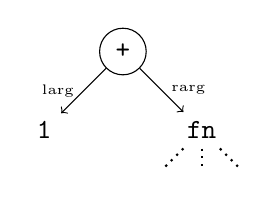
\begin{tikzpicture}
  \node[draw, circle] (plus) at (1,1) {\texttt{+}};
  \node (one) at (0,0) {\texttt{1}};
  \node (fn) at (2,0) {\texttt{fn}};
  \draw[->] (plus) to node[pos=0.5, left, label distance=5mm]{\tiny{larg}} (one);
  \draw[->] (plus) to node[pos=0.5, right, label distance=5mm]{\tiny{rarg}} (fn);
  \draw[dotted, thick] (fn) to +(-0.5, -0.5);
  \draw[dotted, thick] (fn) to +(0, -0.5);
  \draw[dotted, thick] (fn) to +(0.5, -0.5);
  \end{tikzpicture}
  \caption{AST-representation of \texttt{1 + fn(...)}.}
  \label{ast:expr}
\end{wrapfigure}

The \REXPR-rules purpose is to traverse the AST and to analyze each subtree independently. I use the generic term of a \textit{function} to refer to syntactic constructs that consists of a node with multiple subtrees that are independent from each other. Beside built-in functions and UDFs those are operators, aggregates, subquery expressions (eg. \texttt{n IN (...)}), row-comparisons, array-element access, arrays itself and \texttt{VALUES}-lists. The last may be surprising first, but \texttt{(VALUES (1), (2), (3))} or \texttt{ARRAY[1, 2, 3]} is nothing else than a constructor -- a function.

Multiple evaluation scenarios may be obtained for each subtree. These scenarios need to be combined again to return the different evaluation scenarios of the function itself. This is done by building the cross product between the scenarios of each subtree. We obtain all possible combinations of evaluation scenarios of the subtrees, constituting the scenarios of the function (\autoref{fig:expr-expr}).

\begin{figure}[h]
    \centering
    \footnotesize
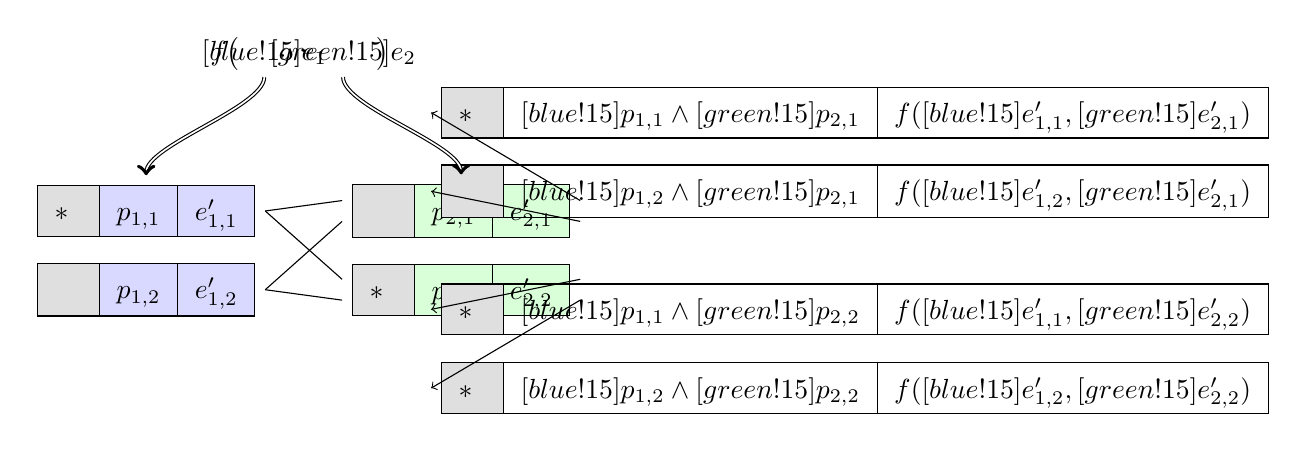
\begin{tikzpicture}[x=10mm, y=10mm]
\node      at (1, 5) {$f\big($};
\node (e1) at (1.5, 5) {$\highlight[blue!15]{e_1}$};
\node      at (2, 5) {$,$};
\node (e2) at (2.5, 5) {$\highlight[green!15]{e_2}$};
\node      at (3, 5) {$\big)$};

\node (e11) at (0, 3) { 
    \begin{tabular}{|p{1em}|r|c|}\hline
    \cellcolor{gray!25} $\ast$ & \cellcolor{blue!15}${p_{1,1}}$ & \cellcolor{blue!15}${e'_{1,1}}$\\\hline
    \end{tabular}
};
\node (e12) at (0, 2) { 
    \begin{tabular}{|p{1em}|r|c|}\hline
    \cellcolor{gray!25}  & \cellcolor{blue!15}${p_{1,2}}$ & \cellcolor{blue!15}${e'_{1,2}}$\\\hline
    \end{tabular}
};

\node (e21) at (4, 3) { 
    \begin{tabular}{|p{1em}|r|c|}\hline
    \cellcolor{gray!25}  & \cellcolor{green!15}${p_{2,1}}$ & \cellcolor{green!15}${e'_{2,1}}$\\\hline
    \end{tabular}
};
\node (e22) at (4, 2) { 
    \begin{tabular}{|p{1em}|r|c|}\hline
    \cellcolor{gray!25}$\ast$ & \cellcolor{green!15}${p_{2,2}}$ & \cellcolor{green!15}${e'_{2,2}}$\\\hline
    \end{tabular}
};

\node (r1) at (9, 4.25) { 
    \begin{tabular}{|p{1em}|r|c|}\hline
    \cellcolor{gray!25} $\ast$ & $\highlight[blue!15]{p_{1,1}} \land \highlight[green!15]{p_{2,1}}$ & $f(\highlight[blue!15]{e'_{1,1}}, \highlight[green!15]{e'_{2,1}})$\\\hline
    \end{tabular}
};
\node (r2) at (9, 3.25) { 
    \begin{tabular}{|p{1em}|r|c|}\hline
    \cellcolor{gray!25}  & $\highlight[blue!15]{p_{1,2}} \land \highlight[green!15]{p_{2,1}}$ & $f(\highlight[blue!15]{e'_{1,2}}, \highlight[green!15]{e'_{2,1}})$\\\hline
    \end{tabular}
};

\node (r3) at (9, 1.75) { 
    \begin{tabular}{|p{1em}|r|c|}\hline
    \cellcolor{gray!25} $\ast$ & $\highlight[blue!15]{p_{1,1}} \land \highlight[green!15]{p_{2,2}}$ & $f(\highlight[blue!15]{e'_{1,1}}, \highlight[green!15]{e'_{2,2}})$\\\hline
    \end{tabular}
};
\node (r4) at (9, 0.75) { 
    \begin{tabular}{|p{1em}|r|c|}\hline
    \cellcolor{gray!25} $\ast$ & $\highlight[blue!15]{p_{1,2}} \land \highlight[green!15]{p_{2,2}}$ & $f(\highlight[blue!15]{e'_{1,2}}, \highlight[green!15]{e'_{2,2}})$\\\hline
    \end{tabular}
};
\draw[->, double, out=270, in=90, looseness = 0.5] (e1.south) to (e11);
\draw[->, double, out=270, in=90, looseness = 0.5] (e2.south) to (e21);

\draw (e11.east) -- (e21.175);
\draw (e11.east) -- (e22.175);
\draw (e12.east) -- (e21.185);
\draw (e12.east) -- (e22.185);

\draw[->] (e21.5) -- (r1.west);
\draw[->] (e21.355) -- (r2.west);
\draw[->] (e22.5) -- (r3.west);
\draw[->] (e22.355) -- (r4.west);
\end{tikzpicture}

    \caption{Operands of a function are translated separately. For each operand a number of scenarios is generated. All possible scenarios of the original function are created by using the cross product.}
    \label{fig:expr-expr}
\end{figure}

\iffalse
$
\inferrule*[Right=(expr)]{
    \inferrule*[Left=(rec)]{ }{
        {\begin{minipage}[b]{15em}
        \mintinline{postgresql}{(TRUE, fib($1 - 1)) ->}
        \mintinline{postgresql}{({}, {(TRUE, fib($1 - 1))})}
        \end{minipage}}
    }\\
    \inferrule*[Right=(rec)]{ }{
        {\begin{minipage}[b]{15em}
        \mintinline{postgresql}{(TRUE, fib($1 - 2)) ->}
        \mintinline{postgresql}{({}, {(TRUE, fib($1 - 2))})}
        \end{minipage}}
    }
}{
    {\begin{minipage}[b]{25em}
    \mintinline{postgresql}{(TRUE, fib($1 - 1) + fib($1 - 2)) ->}
    \mintinline{postgresql}{({}, {(TRUE AND TRUE AND TRUE, fib($1 - 1) + fib($1 - 2))})}
    \end{minipage}}
}
$
\fi

The \REXPR-rule formalizes this idea (\autoref{rule:expr}). $\oplus$ is used as meta-variable for any suitable function etc. Each subtree $e_i$ is translated independently, resulting in the $1 \leq i \leq n$ tuples of scenarios $(B_i, R_i$). Note that the rule is only applicable if at least on subtree contains a callsite, otherwise it would overlap with \RBASE.

\begin{figure}[h!]
    \centering
$$\inferrule{
    \exists i \in \{1, ..., n\}: T \vdash \hasCallsite(e_i)\\
    \forall i \in \{1, ..., n\}: T, C \vdash (\TRUE, e_i) \rightarrow (B_i, R_i)
}{
    T, C \vdash (p, \oplus_{1\leq i \leq n} e_i) \rightarrow \\\\
    {\begin{tabular}[b]{L}
                 \Big( \Big\{(p ~\AND~ (\AND_{1\leq i \leq n} p_i)), \oplus_{1\leq i \leq n} e_i'           ~|~~ ((p_1, e_1'), ..., (p_n, e_n')) \in \times_{\{i|1\leq i \leq n\}} \phantom{(}B_i~~~~~~~~~\Big\}, \\
        \phantom{\Big(}\Big\{(p ~\AND~ (\AND_{1\leq i \leq n} p_i)), \oplus_{1\leq i \leq n} e_i\phantom{'} ~|~~ ((p_1, e_1'), ..., (p_n, e_n')) \in \times_{\{i|1\leq i \leq n\}} (B_i \cup R_i),\\
        \hspace*{58mm}\exists e \in \{e'_1, ..., e'_n\} : \hasCallsite(T, e)~~~~~~~~~~~\Big\}~\Big)
    \end{tabular}}
}\quad(\textsc{expr})$$
    \caption{\REXPR-rule}
    \label{rule:expr}
\end{figure}

Nonrecursive scenarios of the function are created by replacing each argument with the expression from one of its scenarios. The cross product between all nonrecursive scenarios $B_i$ is used to build a set of all possible combinations of nonrecursive scenarios. The predicates $p_i$ of the scenario of each of the $n$ arguments are all unioned by \texttt{AND}. The arguments of the original function is replaced with the expressions generated by the scenarios.

To create all scenarios of the function where at least one argument is recursive, the cross product between all scenarios of an argument (recursive and nonrecursive) is built. Only those combinations where at least one expression is recursive are kept.

To translate entire queries we need to traverse the three different parts of a query: The \texttt{SELECT}-list, the \texttt{FROM}-list and the predicate in \texttt{WHERE}. The idea from the \REXPR-rule applies here as well, but some additionally premises must hold. Only one of the three clauses may be recursive. If the \texttt{WHERE}-clause contains a callsite, any other callsites located elsewhere in the query would depend on that callsites. If a callsite is present in the \texttt{FROM}-list, the execution of the callsites within \texttt{SELECT}- and \texttt{WHERE}-clauses would depend on the callsite in the \texttt{FROM}-list. Therefore, only one of the three parts of a query may contain a callsite.

As of know, there are three different rules to analyze callsites in each clause of a query. In the future, they could be probably combined into an extended version of the \REXPR-rule as all four rules do basically the same.

\begin{figure}[h!]
    \centering
    {\small
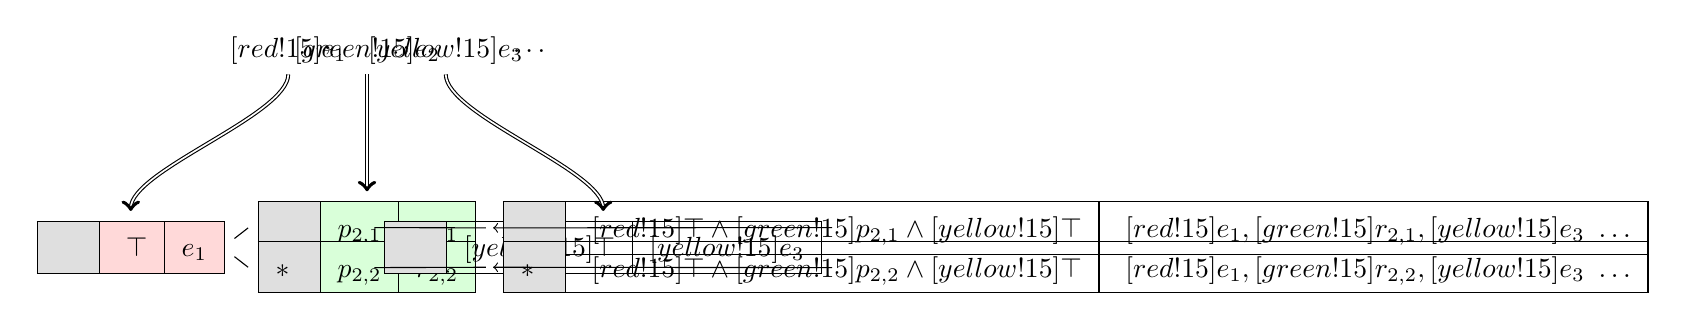
\begin{tikzpicture}[x=5mm, y=5mm]
\node      at ( 8, 9) {$\SELECT$};
\node (e1) at (10, 9) {$\highlight[red!15]{e_1}$};
\node      at (11, 9) {$,$};
\node (e2) at (12, 9) {$\highlight[green!15]{e_2}$};
\node      at (13, 9) {$,$};
\node (e3) at (14, 9) {$\highlight[yellow!15]{e_3}$};
\node      at (16, 9) {$\FROM ~ \dots$};

\node (e11) at (6, 4) { 
    \begin{tabular}{|p{1em}|r|c|}\hline
    \cellcolor{gray!25}  & \cellcolor{red!15} $\top$ & \cellcolor{red!15}$e_1$\\\hline
    \end{tabular}
};

\node (e21) at (12, 4.5) { 
    \begin{tabular}{|p{1em}|r|c|}\hline
    \cellcolor{gray!25}  & \cellcolor{green!15}$p_{2,1}$ & \cellcolor{green!15}$r_{2,1}$\\\hline
    \end{tabular}
};
\node (e22) at (12, 3.5) { 
    \begin{tabular}{|p{1em}|r|c|}\hline
    \cellcolor{gray!25} $\ast$ & \cellcolor{green!15}$p_{2,2}$ & \cellcolor{green!15}$r_{2,2}$\\\hline
    \end{tabular}
};

\node (e31) at (18, 4) { 
    \begin{tabular}{|p{1em}|r|c|}\hline
    \cellcolor{gray!25} & $\highlight[yellow!15]{\top}$ & $\highlight[yellow!15]{e_3}$\\\hline
    \end{tabular}
};

\node (r1) at (30, 4.5) { 
    \begin{tabular}{|p{1em}|r|c|}\hline
    \cellcolor{gray!25}  & $\SELECT ~ \highlight[red!15]{\top} \land \highlight[green!15]{p_{2,1}} \land \highlight[yellow!15]{\top}$ & $\SELECT~ \highlight[red!15]{e_1}, \highlight[green!15]{r_{2,1}}, \highlight[yellow!15]{e_3} ~ \FROM \dots$\\\hline
    \end{tabular}
};
\node (r2) at (30, 3.5) { 
    \begin{tabular}{|p{1em}|r|c|}\hline
    \cellcolor{gray!25} $\ast$ & $\SELECT ~ \highlight[red!15]{\top} \land \highlight[green!15]{p_{2,2}} \land \highlight[yellow!15]{\top}$ & $\SELECT~ \highlight[red!15]{e_1}, \highlight[green!15]{r_{2,2}}, \highlight[yellow!15]{e_3} ~ \FROM \dots$\\\hline
    \end{tabular}
};
\draw[->, double, out=270, in=90, looseness = 0.5] (e1.south) to (e11);
\draw[->, double, out=270, in=90, looseness = 0.5] (e2.south) to (e21);
\draw[->, double, out=270, in=90, looseness = 0.5] (e3.south) to (e31);
\draw (e11.5) to (e21.west);
\draw (e11.355) to (e22.west);
\draw (e21.east) to (e31.175);
\draw (e22.east) to (e31.185);
\draw[->] (e31.5) -- (r1.west);
\draw[->] (e31.355) -- (r2.west);
%\draw[->, bend left=20]  (e11.north) to (e21.north) to (e31.north) to (r1.west);
%\draw[->, bend right=20] (e11.south) to (e22.south) to (e31.south) to (r2.west);
\end{tikzpicture}}
    \caption{The projection of a relation happening inside \SELECT~can be understood as a function $\SELECT(e_1, \dots, e_n, T)$. The same happens analogously for the \FROM-clause: $\FROM(T_1, \dots, T_m)$}
    \label{fig:expr-select}
\end{figure}

The idea how to analyze queries with callites in the select-list follows directly the idea of the \REXPR-rule (\autoref{fig:expr-select}). Each target from the \texttt{SELECT}-list is analyzed independently and used to reconstruct the actual \texttt{SELECT}. Other parts of the query are unchanged and will not analyzed at all, since they must be nonrecursive.

The inference rule (\autoref{rule:select}) is nearly identical to the \REXPR-rule, only additional premises enforce the constraints stated above. Another difference is, that the "function" representing the query is not entirely analyzed but only the \texttt{SELECT}-clause. Other clauses do not contain callsites and would lead to the application the \RBASE-rule, leaving them unchanged.

\begin{figure}[h!]
    \centering\footnotesize
  \makebox[\textwidth][c]{
$$\inferrule{
    \exists i \in \{1, ..., n\}: T \vdash \hasCallsite(e_i) \\
    \neg \hasCallsite(T, ts) \\
    \neg \hasCallsite(T, w) \\\\
    \forall i \in \{1, ..., n\}: T, \varnothing \vdash (\TRUE, e_i) \rightarrow (B_i, R_i)
}{
    T, \varnothing \vdash (p, \SELECT~ e_1, ..., e_n ~\FROM ~ts ~\WHERE~w) \rightarrow \\\\
    {\begin{tabular}[b]{L}
             \Big( \big\{\big(\SELECT~ p ~\AND~ p_1 ~\AND~ \cdots ~\AND~ p_n, ~\SELECT~ e'_1, ..., e'_n ~\FROM ~ts~\WHERE ~w \big) | ~((p_1, e'_1), ..., (p_n, e'_n)) \in \times_{1 \leq i \leq n} B_i~~~~~~~~~\big\}, \\
    \phantom{\Big(}\big\{\big(\SELECT~ p ~\AND~ p_1 ~\AND~ \cdots ~\AND~ p_n,~ \SELECT~ e'_1, ..., e'_n ~\FROM ~ts~ \WHERE~w \big) | ~((p_1, e'_1), ..., (p_n, e'_n)) \in \times_{1 \leq i \leq n} (B_i \cup R_i),\\
    \hspace{104mm}\exists e \in \{e'_1, ..., e'_n\} : \hasCallsite(T, e)~~~~~~\big\}\Big)\\
    \end{tabular}}
}
\quad(\textsc{select})$$}
    \caption{\RSELECT-rule}
    \label{rule:select}
\end{figure}




A recursive \texttt{FROM}-clause works analogously, the \RFROM-rule is nearly identical \RSELECT-rule (\autoref{rule:from}). Instead of the \texttt{SELECT}-list, the \texttt{FROM}-list is analyzed. Other parts of the query cannot contain callsites and are left therefore unchanged.

\begin{figure}[h!]
    \centering\footnotesize
  \makebox[\textwidth][c]{
$$\inferrule{
    \exists i \in \{1, ..., n\}: T \vdash \hasCallsite(e_i) \\
    \neg \hasCallsite(T, ts) \\
    \neg \hasCallsite(T, w) \\\\
    \forall i \in \{1, ..., n\}: T, \varnothing \vdash (\TRUE, e_i) \rightarrow (B_i, R_i)
}{
    T, \varnothing \vdash (p, \SELECT~ ts ~\FROM ~e_1, ..., e_n ~\WHERE~w) \rightarrow \\\\
    {\begin{tabular}[b]{L}
             \Big( \big\{\big(\SELECT~ p ~\AND~ p_1 ~\AND~ \cdots ~\AND~ p_n, ~\SELECT ~ts~ \FROM ~e'_1, ..., e'_n~\WHERE ~w \big) | ~((p_1, e'_1), ..., (p_n, e'_n)) \in \times_{1 \leq i \leq n} B_i~~~~~~~~~\big\}, \\
    \phantom{\Big(}\big\{\big(\SELECT~ p ~\AND~ p_1 ~\AND~ \cdots ~\AND~ p_n,~ \SELECT ~ts~ \FROM ~e'_1, ..., e'_n~ \WHERE~w \big) | ~((p_1, e'_1), ..., (p_n, e'_n)) \in \times_{1 \leq i \leq n} (B_i \cup R_i),\\
    \hspace{104mm}\exists e \in \{e'_1, ..., e'_n\} : \hasCallsite(T, e)~~~~~~\big\}\Big)\\
    \end{tabular}}
}
\quad(\textsc{from})$$}
    \caption{\RFROM-rule}
    \label{rule:from}
\end{figure}


\iffalse
\begin{figure}[h!]
    \centering\footnotesize
  \makebox[\textwidth][c]{
$$\inferrule{
    \exists i \in \{1, ..., n\}: \hasCallsite(T, e_{f_i}) \\
    \neg \hasCallsite(T, ts)\\
    \neg \hasCallsite(T, w) \\\\
    \forall i \in \{1, ..., n\}: T, \varnothing \vdash (\TRUE, t_i) \rightarrow (B_i, R_i)
}{
T, \varnothing \vdash (p, \SELECT~ ts ~\FROM~ t_1 \AS a_1 \otimes ... \otimes  t_n \AS a_n ~\WHERE~ w) \rightarrow \\\\
{\begin{tabular}[b]{LLLL}
         \Big( \big\{ (\SELECT~ p ~\AND~ p_1 ~\AND~ \cdots ~\AND~ p_n,~ \SELECT~ ts ~\FROM~ t'_1 \AS a_1 \otimes ... \otimes  t'_n \AS a_n ~\WHERE~ w ~~)\\
\phantom{\Big( \big\{}| ~((p_1, t'_1), ..., (p_n, t'_n)) \in \times_{\{i|1\leq i \leq n\}} B_i \hspace*{80mm}\big\}, \\
\phantom{\Big(}\big\{ (\SELECT~ p ~\AND~ p_1 ~\AND~ \cdots ~\AND~ p_n,~ \SELECT~ ts ~\FROM~ t'_1 \AS a_1 \otimes ... \otimes  t'_n \AS a_n ~\WHERE~ w ~~)\\
\phantom{\Big( \big\{}| ~ ((p_1, t'_1), ..., (p_n, t'_n)) \in \times_{\{i|1\leq i \leq n\}} (B_i \cup R_i), \exists t' \in \{t'_1, ..., t'_n\} : \hasCallsite(t') \hspace*{17mm}\big\}\Big)\\
\end{tabular}}
}
\quad(\textsc{from})
$$
}
    \caption{\RFROM-rule}
    \label{rule:from}
\end{figure}
\fi

Finally, the callsite may be located inside the where-clause of the query. The \RWHERE-rule (\autoref{rule:where}) is is simpler because there is just a single expression that need to be analyzed and replaced in the query. Other parts of the query do not have to be considered.

%Probably all three rules to handle queries could be combined into a single rule. The premises would need to enforce that exactly one of the three parts contains a callsite and the actual rule would analyze all parts of the query. If we augment the \REXPR-rule with appropriate premises, all three rules could probably be replaced by the \REXPR-rule.

\begin{figure}[h!]
    \centering\small
  \makebox[\textwidth][c]{
$$\inferrule{
    \neg \hasCallsite(T, ts) \\
    \neg \hasCallsite(T, es) \\
    \hasCallsite(T, w) \\\\
    T, \varnothing \vdash (p, w) \rightarrow (B, R)
}{
    T, \varnothing \vdash (p, \SELECT~ es ~\FROM ~ts~ \WHERE~w) \rightarrow \\\\
    {\begin{tabular}[b]{L}
             \Big( \big\{\big(\SELECT~ p', ~\SELECT ~es~ \FROM ~ts~ \WHERE ~w' \big) | ~(p', w') \in B\big\}, \\
    \phantom{\Big(}\big\{\big(\SELECT~ p', ~\SELECT ~es~ \FROM ~ts~ \WHERE ~w' \big) | ~(p', w') \in R\big\}\Big)\\
    \end{tabular}}
}
\quad(\textsc{where})$$}
    \caption{\RWHERE-rule}
    \label{rule:where}
\end{figure}


\iffalse
$$\quad(\textsc{where})\inferrule{
    T \vdash \neg \hasCallsite(e_{s}) \\
    \forall i \in \{1 \leq i \leq n\} : T \vdash \neg \hasCallsite(e_{t_i}) \\
    T \vdash \hasCallsite(e_{w}) \\
    T, \varnothing \vdash (p, e_{w}) \rightarrow (B, R)
}{
    T, \varnothing \vdash (p, \SELECT~ e_s ~\FROM~ t_1 ~\AS~ a_1 \otimes ... \otimes t_n ~\AS~ a_n ~\WHERE~ e_w) \rightarrow \\\\
    {\begin{tabular}[b]{LLLL}
    (~~&\{&(&\SELECT~ p_w  ~\FROM~ t_1 ~\AS~ a_1 \otimes ... \otimes  t_n ~\AS~ a_n ~\WHERE~ e'_w,\\
        &&&\SELECT~ e_s ~\FROM~ t_1 ~\AS~ a_1 \otimes ... \otimes  t_n ~\AS~ a_n ~\WHERE~ e'_w~~) \\
        && | &~(p_w, e'_w) \in B~~\}, \\
     &\{&(&\SELECT~ p_w ~\FROM~ t_1 ~\AS~ a_1 \otimes ... \otimes  t_n ~\AS~ a_n ~\WHERE~ e'_w, \\
        &&&\SELECT~ e_s ~\FROM~ t_1 ~\AS~ a_1 \otimes ... \otimes  t_n ~\AS~ a_n ~\WHERE~ e'_w~~) \\
        && | &~(p_w, e'_w) \in R~~\}~~)\\
    \end{tabular}}
}$$
\begin{figure}[h!]
    \centering
    {\small
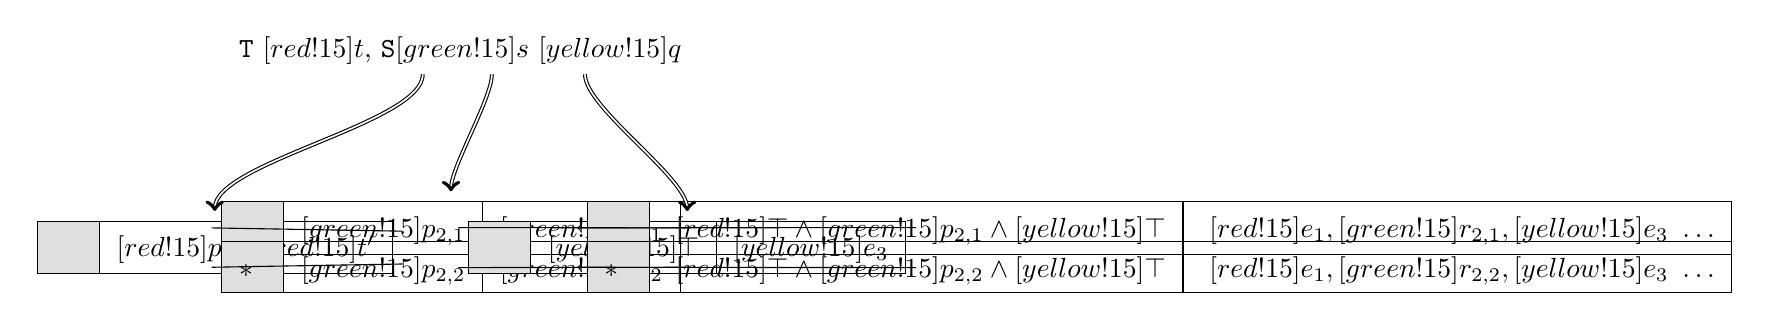
\begin{tikzpicture}[x=5mm, y=5mm, node distance=1mm]
\node (ctes) at (12,9) {\WITH~ \texttt{T} \AS $\highlight[red!15]{t}$, \texttt{S}\AS $\highlight[green!15]{s}$ $\highlight[yellow!15]{q}$};

\node (e11) at (6, 4) { 
    \begin{tabular}{|p{1em}|r|c|}\hline
    \cellcolor{gray!25}  & $\highlight[red!15]{p_t}$ & $\highlight[red!15]{t'}$\\\hline
    \end{tabular}
};

\node (e21) at (12, 4.5) { 
    \begin{tabular}{|p{1em}|r|c|}\hline
    \cellcolor{gray!25}  & $\highlight[green!15]{p_{2,1}}$ & $\highlight[green!15]{r_{2,1}}$\\\hline
    \end{tabular}
};
\node (e22) at (12, 3.5) { 
    \begin{tabular}{|p{1em}|r|c|}\hline
    \cellcolor{gray!25} $\ast$ & $\highlight[green!15]{p_{2,2}}$ & $\highlight[green!15]{r_{2,2}}$\\\hline
    \end{tabular}
};

\node (e31) at (18, 4) { 
    \begin{tabular}{|p{1em}|r|c|}\hline
    \cellcolor{gray!25} & $\highlight[yellow!15]{\top}$ & $\highlight[yellow!15]{e_3}$\\\hline
    \end{tabular}
};

\node (r1) at (30, 4.5) { 
    \begin{tabular}{|p{1em}|r|c|}\hline
    \cellcolor{gray!25}  & $\SELECT ~ \highlight[red!15]{\top} \land \highlight[green!15]{p_{2,1}} \land \highlight[yellow!15]{\top}$ & $\SELECT~ \highlight[red!15]{e_1}, \highlight[green!15]{r_{2,1}}, \highlight[yellow!15]{e_3} ~ \FROM \dots$\\\hline
    \end{tabular}
};
\node (r2) at (30, 3.5) { 
    \begin{tabular}{|p{1em}|r|c|}\hline
    \cellcolor{gray!25} $\ast$ & $\SELECT ~ \highlight[red!15]{\top} \land \highlight[green!15]{p_{2,2}} \land \highlight[yellow!15]{\top}$ & $\SELECT~ \highlight[red!15]{e_1}, \highlight[green!15]{r_{2,2}}, \highlight[yellow!15]{e_3} ~ \FROM \dots$\\\hline
    \end{tabular}
};
\draw[->, double, out=270, in=90, looseness = 0.5] (ctes.220) to (e11);
\draw[->, double, out=270, in=90, looseness = 0.5] (ctes.330) to (e21);
\draw[->, double, out=270, in=90, looseness = 0.5] (ctes.350) to (e31);
\draw (e11.5) to (e21.west);
\draw (e11.355) to (e22.west);
\draw (e21.east) to (e31.175);
\draw (e22.east) to (e31.185);
\draw[->] (e31.5) -- (r1.west);
\draw[->] (e31.355) -- (r2.west);
%\draw[->, bend left=20]  (e11.north) to (e21.north) to (e31.north) to (r1.west);
%\draw[->, bend right=20] (e11.south) to (e22.south) to (e31.south) to (r2.west);
\end{tikzpicture}}
    \caption{The ~\WITH-clause could also be viewed as composition of functions $\WITH(t, T, q)$ that binds a table-variable \texttt{T} to an expression \texttt{t} for a given query \texttt{q}. In this example it would be $\WITH(T, t, \WITH(S, s, q))$ as CTEs can reference preceding ones.}
    \label{fig:expr-cte}
\end{figure}

\sqlcode[mathescape=true]{snippets/rule_from_example.sql}


$
\inferrule*{
    \inferrule*{...}{
{\begin{minipage}[b]{12em}
\sqlcode{snippets/rules/fib/01-case.sql}
\end{minipage}}
    }
}{
{\begin{minipage}[b]{12em}
\sqlcode{snippets/rules/fib/01-select.sql}
\end{minipage}}
}
$

\fi

\subsection{Examples}


\section{Handling CTEs}

Common Table Expressions (CTEs) are a powerful tool to structure and tweak complex queries. They work like temporary tables that only exist for an individual query. But allowing CTEs that may contain callsites introduce some complexities that need to be considered when analyzing.

% Without CTEs hasCallsite just checks the subtree
With S-F-W queries the notion of \textit{containing a callsite} (or being \textit{recursive}) is simple. If a query-fragment $e$ contains a callsite, the subexpression is recursive: $\hasCallsite(e) = fn \sqsubset e$. From an implementation point of view, it is as simple as filtering the AST of $e$ for callsites.

\begin{wrapfigure}{r}{.5\textwidth} 
    \begin{minipage}{\linewidth}
    \label{fig:simple_indiref}\par\vfill
    \begin{minted}{postgresql}
    WITH S AS (SELECT f(n-1)),
         T AS (SELECT * FROM S)
    SELECT * FROM T
    \end{minted}
    \subcaption{Neither the actual query nor the referenced CTE \texttt{T} directly contains a callsite.}
    \label{fig:indirect_callsite}\par
    \vspace{3mm}
    \begin{minted}{postgresql}
    SELECT (
        WITH T AS (SELECT f(n-1))
        SELECT 1
    )
    \end{minted}
    \subcaption{Our definition of $\hasCallsite$ would fail here since a callsite is located in the subtree. The query is acutally nonrecursive.}
    \label{fig:unused_callsite}
\end{minipage}
\caption{}
\label{lst:indirect_callsite_ref}\vspace{-5mm} 
\end{wrapfigure}

% CTEs introduce indirect callsites that make callsite detection more complicated
With CTEs we need to consider two additional issues. First, callsites can now be located outside the current subtree by referencing recursive CTEs (\autoref{fig:indirect_callsite}). Second, a scenario may contain unused recursive CTEs, fooling $\hasCallsite$ as stated above to believe a given query-fragment is recursive, even if the recursive CTEs are unused and thus never evaluated (\autoref{fig:unused_callsite}).

% Removing all CTEs, translating then and then reattaching only used CTEs fixes this.
We can counter this issues, if we remove the CTEs from the original query before translating the actual query. For each query-scenario only those scenarios of CTEs are reattached afterwards that are actually used (\autoref{tracking_recursive_ctes}). To detect indirect callsite references, we note recursive CTEs in a list when detaching (\autoref{tracking_cte_dependencies}) and check against that list if we encounter free table-variables in the query.

\subsection{Tracking recursive CTEs}\label{tracking_recursive_ctes}

% Recursive CTEs are gathered step by step 
CTEs may contain callsites and therefore need to be analyzed too. They are processed step by step before the actual query. This enables a CTE to reference preceeding CTEs. If a CTE-scenario contains a callsite, its alias is added to the list of recursive CTEs $T$ in scope. Otherwise, the alias is removed from that list because the new CTE shadows any outer recursive CTE with the same name (\texttt{WITH}-queries can be nested). (\autoref{lst:indirect_callsite_ref}).

Whenever an query-fragment is encountered that references a CTE from $T$, we know that this fragment is recursive. This way, we can build up $T$ incrementally and do not need to track each reference recursively back to its declaration to find out whether its recursive. For an example see \autoref{fig:tracking_recursive_ctes}.

\begin{figure}[h]
    \small
    \centering
    \begin{tikzpicture}[x=8mm, y=8mm]
    \node at (0.5, 1) {\footnotesize{(a)}};
    \node at (5.5, 1) {\footnotesize{(b)}};
    \node at (15.5, 1) {\footnotesize{(c)}};
    \node[anchor=west] at (-1, 0) {\WITH};
    \node[anchor=west] (A) at (0, 0)  {\texttt{A} \AS $(\ast a),$};
    \node[anchor=west] (B) at (0, -1) {\texttt{B} \AS $(b),$};
    \node[anchor=west] (C) at (0, -2) {\texttt{C} \AS $(c),$};
    \node[anchor=west] (D) at (0, -3) {\texttt{D} \AS $(d)$};
    \node[anchor=north west] (S) at (-1, -3.75) {$\underbrace{\SELECT~\texttt{*}~\FROM~\texttt{D}}_q$};
    \node[anchor=west] (Ar) at (3, 0)  {$fn \sqsubset a  \Longrightarrow  \hasCallsite(T, q)$};
    \node[anchor=west] (Br) at (3, -1) {$\FV(b) \cap T = \emptyset \cap \{\texttt{A}\} = \emptyset  \Longrightarrow  \neg \hasCallsite(T, q)$};
    \node[anchor=west] (Cr) at (3, -2) {$\FV(c) \cap T = \{A\} \cap \{A\} \neq \emptyset  \Longrightarrow  \hasCallsite(T, q)$};
    \node[anchor=west] (Dr) at (3, -3) {$\FV(d) \cap T = \{C\} \cap \{A, C\} \neq \emptyset  \Longrightarrow  \hasCallsite(T, q)$};
    \node[anchor=north west] (Dr) at (3, -3.75) {$\FV(q) \cap T = \{D\} \cap \{A, C, D\} \neq \emptyset  \Longrightarrow  \hasCallsite(T, q)$};
    \node[anchor=west] (Ar) at (13.5, 0) {$T := T \cup \{\texttt{A}\} = \{\texttt{A}\}$};
    \node[anchor=west] (Br) at (13.5, -1) {$T := T \setminus \{\texttt{B}\} = \{\texttt{A}\}$};
    \node[anchor=west] (Cr) at (13.5, -2) {$T := T \cup \{\texttt{C}\} = \{\texttt{A}, \texttt{C}\}$};
    \node[anchor=west] (Dr) at (13.5, -3) {$T := T \cup \{\texttt{D}\}= \{\texttt{A}, \texttt{C}, \texttt{D}\}$};
    \draw[->, bend right=60] (C) to (A);
    \draw[->] (C) to (B);
    \draw[->] (D) to (C);
    \end{tikzpicture}
    \caption{a) $q$ has no direct callsite, but reference \texttt{D} that contains a reference to \texttt{A} via \texttt{C}. \texttt{A} contains a direct callsite. b) A fragment $e$ is considered recursive if it contains a direct callsite ($fn \sqsubset$ e) or uses a recursive table-variable. c) If $\hasCallsite$ yields true for a CTE-body, its alias is added to the set of recursive table-variables $T$. Otherwise, the alias is removed to take into account shadowing.}
    \label{fig:tracking_recursive_ctes}
\end{figure}

% Referenced CTEs are detected via unbound variables
References to CTEs can be easily collected from a query-fragment by searching for free table-variables. The function to compute all free table-variables of a query-fragment $e$ is called $\FV(e)$. Its implemention is straight forward: Each CTE definition within a \WITH-block adds its alias to the list of bound table-variables. Every reference to a table-variable that is not contained in that list is considered free.

\begin{wrapfigure}{r}{0.4\textwidth}
    \begin{minted}{postgresql}
    WITH T AS (SELECT fn(n-1))
    SELECT *
    FROM (
      WITH T AS (SELECT 1)
      SELECT * FROM T
    ) T
    \end{minted}
    \caption{The outer, recursive CTE \texttt{T} is shadowed by an inner CTE.}
    \label{lst:indirect_callsite_ref}
\end{wrapfigure}

% Row-references vs. table-variables
Note that there can occur two different types of free variables inside a query-fragment: \textit{Table-Variables} and \textit{Row-References}. Table-variables like \texttt{T} can exclusively be used in ~\FROM~ and reference an entire table. This table-variables are introduced either by the existence of a table in the current database or by an CTE. Row-references like \texttt{T.v} point to a single table-row of a table referenced by ~\FROM. A bare row-reference cannot cause a query to be recursive, it is always the from-clause that declares this row-references and binds it to a table. This table is always evaluated first, no matter of any row-reference is used at all. For this reason it is sufficient to track only \textit{table}-variables and ignore row-references entirely.

As we now know which CTEs in scope are recursive, we can reformulate the function to determine whether a query-fragment contains a callsite directly or via a reference:
$$\hasCallsite(T, e) = fn(\dots) \sqsubset e \lor \FV(e) \cap T \neq \emptyset$$
Either the callsite is directly contained in $e$, or it contains a free table-variable that is also enlisted in $T$. Otherwise the query-fragment is not recursive.

With indirect references, we need another axiom for recursive references:

% REF
$$\quad(\textsc{ref})\inferrule{
   \text{isReference}(S) \\
   T \vdash \hasCallsite(S)
}{
    T, C \vdash (p, S) \rightarrow (\{\}, \{(p, S)\})
}$$

%We process CTEs of a \WITH-block top down, before translating the actual \SELECT-query, resembling the way SQL evaluates them. If a CTE \texttt{T} references a CTE \texttt{S} that is recursive, \texttt{T} is also recursive. SQL evaluates CTEs in the order they are defined, so that preceding CTEs can be referenced by following CTEs (figure 4.4a FIXME?). Furthermore, CTEs can be nested so that we need to take care of shadowing out outer CTEs.

%Instead of tracing every reference through the entire query until the initial definition is found, I take an incremental approach: If a new table-variable is created, we check each free variable in its subtree against the environment of known recursive table-references within that scope. If there is a recursive table referenced or the subtree contains an immediate recursive call, the new table-reference is entailed the set of recursive table-references.

%Each CTE-scenario is augmented with its dependencies to previously defined CTEs. Each CTE is sliced into its different scenarios, then each scenario is analyzed, removed from the query and stored in the queue. When all CTEs are processed and the actual query is translated, only those CTEs are reattached to the query-scenario that are actually used. Indirect callsites can be detected by simply checking if there exists a free table-variable that is enlisted in $T$.

\subsection{Tracking CTE-dependencies}\label{tracking_cte_dependencies}
As we have seen, CTEs may use other CTEs so that we need to keep track of the dependencies of a scenario. This happens similar to the creation of the set $T$ of recursive CTEs. For each CTE \texttt{C} we collect all its CTE-references \texttt{$C_i$} from the scenario (predicate and query) together with their dependencies. For an illustration see \autoref{fig:cte_deps}.

\iffalse
\begin{figure}[h!]
    \centering
    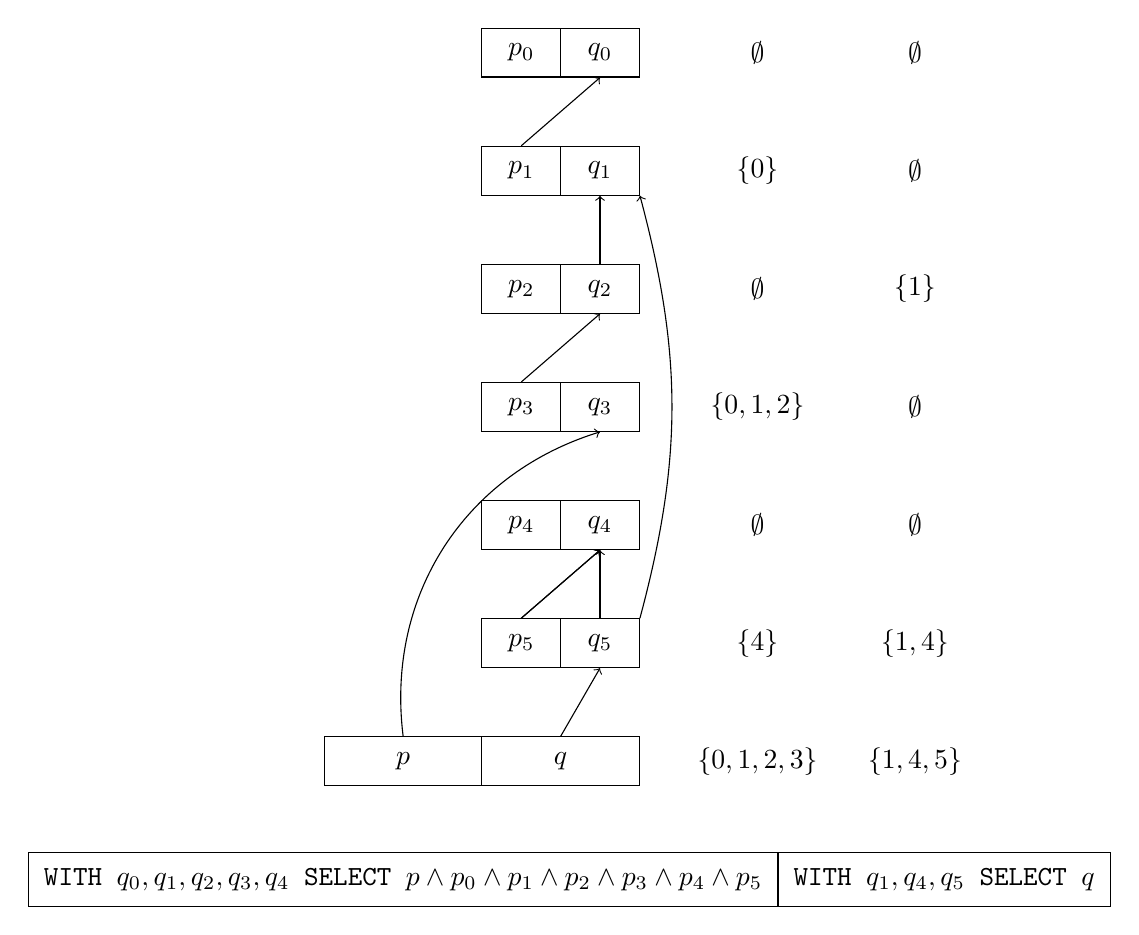
\begin{tikzpicture}[x=10mm, y=15mm, node distance=1cm]
    \tikzset{Box/.style={shape=rectangle, draw, minimum width=1cm, minimum height=0.5cm, inner sep=2mm}}
    \node[anchor=west] at (-2.5, 1) {\WITH};
    
    \node[Box] (p0) at (0, 1)  {$p_0$};
    \node[Box, right of=p0] (q0) {$q_0$};
    \node at (3, 1) {$\emptyset$};
    \node at (5, 1) {$\emptyset$};
    
    \node[Box] (p1) at (0, 0)  {$p_1$};
    \node[Box, right of=p1] (q1) {$q_1$};
    \node at (3, 0) {$\{0\}$};
    \node at (5, 0) {$\emptyset$};
    
    \node[Box] (p2) at (0, -1)  {$p_2$};
    \node[Box, right of=p2] (q2) {$q_2$};
    \node at (3, -1) {$\emptyset$};
    \node at (5, -1) {$\{1\}$};
    
    \node[Box] (p3) at (0, -2)  {$p_3$};
    \node[Box, right of=p3] (q3) {$q_3$};
    \node at (3, -2) {$\{0, 1, 2\}$};
    \node at (5, -2) {$\emptyset$};
    
    \node[Box] (p4) at (0, -3)  {$p_4$};
    \node[Box, right of=p4] (q4) {$q_4$};
    \node at (3, -3) {$\emptyset$};
    \node at (5, -3) {$\emptyset$};
    
    \node[Box] (p5) at (0, -4)  {$p_5$};
    \node[Box, right of=p5] (q5) {$q_5$};
    \node at (3, -4) {$\{4\}$};
    \node at (5, -4) {$\{1, 4\}$};
    
    \node[Box, minimum width=2cm] (p) at (-1.5, -5){$p$};
    \node[Box, minimum width=2cm] (q) at (0.5, -5) {$q$};
    \node at (3, -5) {$\{0, 1, 2, 3\}$};
    \node at (5, -5) {$\{1, 4, 5\}$};
    
    \node[Box, minimum width=7cm] (r) at (-1.5, -6){\texttt{WITH $q_0, q_1, q_2, q_3, q_4$ SELECT $p \land p_0 \land p_1 \land p_2 \land p_3 \land p_4 \land p_5$}};
    \node[Box] at (5.37, -6) {\texttt{WITH $q_1, q_4, q_5$ SELECT $q$}};
    
    \draw[->] (p1.north) to (q0.south);
    \draw[->] (q2.north) to (q1.south);
    \draw[->] (p5.north) to (q4.south);
    \draw[->] (p3.north) to (q2.south);
    \draw[->, bend left=40, in=140] (p.north) to (q3.south);
    \draw[->] (p5.north) to (q4.south);
    \draw[->, bend right=15] (q5.north east) to (q1.south east);
    \draw[->] (q.north) to (q5.south);
    \draw[->] (q5.north) to (q4.south);
    \end{tikzpicture}
    \caption{References are tracked incrementally by collecting free table-variables (ie. direct CTE references) along with the references of those free table-variables. Note that the use of $\deps$ here varies from its definition to illustrate the process more clearly.}
    \label{fig:cte_deps}
\end{figure}
\fi

\begin{figure}[h!]
    \centering
    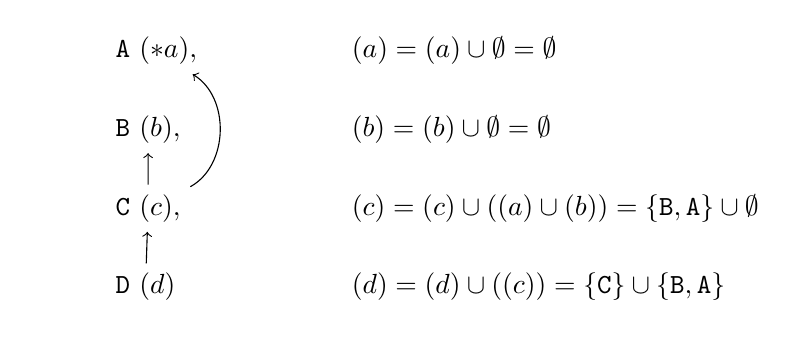
\begin{tikzpicture}[x=10mm, y=10mm]
    \node[anchor=west] at (-1, 0) {\WITH};
    \node[anchor=west] (A) at (0, 0)  {\texttt{A} \AS $(\ast a),$};
    \node[anchor=west] (B) at (0, -1) {\texttt{B} \AS $(b),$};
    \node[anchor=west] (C) at (0, -2) {\texttt{C} \AS $(c),$};
    \node[anchor=west] (D) at (0, -3) {\texttt{D} \AS $(d)$};
    \node[anchor=west] (Ar) at (3, 0)  {$\deps(a) = \FV(a) \cup \emptyset = \emptyset$};
    \node[anchor=west] (Br) at (3, -1) {$\deps(b) = \FV(b) \cup \emptyset = \emptyset$};
    \node[anchor=west] (Cr) at (3, -2) {$\deps(c) = \FV(c) \cup (\deps(a) \cup \deps(b)) = \{\texttt{B}, \texttt{A}\} \cup \emptyset$};
    \node[anchor=west] (Dr) at (3, -3) {$\deps(d) = \FV(d) \cup (\deps(c)) = \{\texttt{C}\} \cup \{\texttt{B}, \texttt{A}\}$};
    \draw[->, bend right=60] (C) to (A);
    \draw[->] (C) to (B);
    \draw[->] (D) to (C);
    \end{tikzpicture}
    \caption{References are tracked incrementally by collecting free table-variables (ie. direct CTE references) along with their dependencies. $a \rightarrow b$ means that $a$ contains a reference to $b$. Note that $\deps$ is simplified here to illustrate the process more clearly.}
    \label{fig:cte_deps}
\end{figure}

The actual implementation differs from the example shown in \autoref{fig:cte_deps}. Each CTE is removed from the query after it is analyzed, therefore it is difficult to trace references recursively back. The ordering of CTEs enables us to perform this task incrementally, creating a full list of dependencies for every individual CTE while analyzing:

$$\deps(C, q) := \FV(q) \cup \left(\bigcup_{(\_, \_, \_, ds) \in C[\FV(q)]} ds \right)$$

The function $\deps$ collects free table-variables (ie. used CTEs) of $q$ together with their dependencies $ds$. CTE-dependencies are retrieved from the CTE-store $C$ using the CTEs used by $q$. Because CTEs cannot make forward-references, we obtain this way a full list of CTE-dependencies.

%Different to tracking recursive CTEs, shadowing is not an issue here. The difference is that the list of recursive table-variables $T$ was passed down to further computation steps. Here, $C$ is only nonempty while processing CTEs of the same \texttt{WITH}-query where CTE-names are unique. Nested CTEs may shadow out outer CTEs indeed, but this issue is already solved by $\FV$.

\iffalse
\begin{figure}[h!]
    \centering
    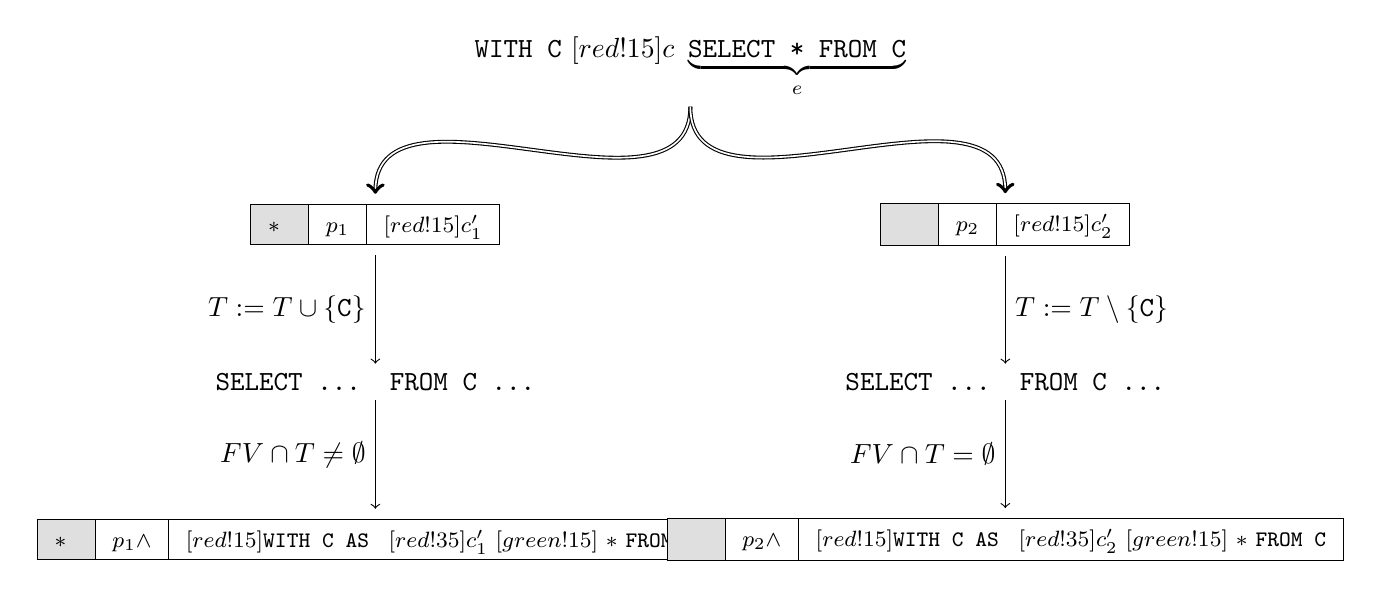
\begin{tikzpicture}
    \node (cte) at (4, 1) {\texttt{WITH C} \AS $\highlight[red!15]{c}~ \underbrace{\texttt{SELECT * FROM C}}_e$};
    \node (cte1) at (0, -1) {\footnotesize
        \begin{tabular}{|p{1em}|r|c|}\hline
        \cellcolor{gray!25} $\ast$ & $p_1$ & $\highlight[red!15]{c'_1}$\\\hline
        \end{tabular}
    };
    \node (cte2) at (8, -1) {\footnotesize
        \begin{tabular}{|p{1em}|r|c|}\hline
        \cellcolor{gray!25} & $p_2$ & $\highlight[red!15]{c'_2}$\\\hline
        \end{tabular}
    };
    \node (select1) at (0, -3) {\texttt{SELECT ... FROM C ...}};
    \node (select2) at (8, -3) {\texttt{SELECT ... FROM C ...}};
    \node (r1) at (0, -5) {\footnotesize
        \begin{tabular}{|p{1em}|r|c|}\hline
        \cellcolor{gray!25} $\ast$ & $p_1 \land \hdots$ & $\highlight[red!15]{\texttt{WITH C AS } ~\highlight[red!35]{c'_1}}~\highlight[green!15]{\SELECT~*~\texttt{FROM C}}$\\\hline
        \end{tabular}
    };
    \node (r2) at (8, -5) {\footnotesize
        \begin{tabular}{|p{1em}|r|c|}\hline
        \cellcolor{gray!25} & $p_2 \land \hdots$ & $\highlight[red!15]{\texttt{WITH C AS } ~\highlight[red!35]{c'_2}}~\highlight[green!15]{\SELECT~*~\texttt{FROM C}}$\\\hline
        \end{tabular}
    };
    \draw[->, double, out=270, in=90] (cte) to (cte1.north);
    \draw[->, double, out=270, in=90] (cte) to (cte2.north);
    \draw[->] (cte1.south) --node[left] {$T := T \cup \{\texttt{C}\}$} (select1);
    \draw[->] (cte2.south) --node[right]{$T := T \setminus \{\texttt{C}\}$} (select2);
    \draw[->] (select1) --node[left] {$FV \cap T \neq \emptyset$} (r1);
    \draw[->] (select2) --node[left] {$FV \cap T = \emptyset$} (r2);
    \end{tikzpicture}
    \caption{}
    \label{fig:my_label}
\end{figure}
\fi

\subsection{{\normalfont\RCTE}-rule: Collecting and analyzing CTE-Scenarios}

The idea from the \REXPR-rule of building the cross product between all scenarios of its subtrees is also present in the \RCTE-rule. Yet, our extended notion of a function does not work the entire \texttt{WITH}-clause. There is no \texttt{WITH}-"function" node at the root with $n$ independent children, one for each CTE: $\texttt{WITH}(t_1, t_2, t_3, q)$. Its more a right-deep tree of individual CTE-definitions where each CTE depends on the preceeding CTEs: $\texttt{CTE}(t_1, \texttt{CTE}(t_2, \texttt{CTE}(t_3, q)))$. Therefore each \texttt{CTE} must be analyzed individually and the environment is modified for accordingly for every CTE-scenario. With the changed environment, following CTEs are analyzed and eventually the actual query $q$.

The environment is changed in two ways: First, the list of recursive table-variables $T$ is updated. If the evaluation-scenario of the CTE is recursive, the alias of the CTE is added to $T$. If the CTE-scenario is nonrecursive, the alias is removed from $T$ since any recursive reference is now shadowed by this nonrecursive CTE. Second, the CTE-scenario is added alongside its dependencies to the CTE-store $C$.

\begin{figure}[h!]
    \centering\footnotesize
\makebox[\textwidth][c]{
$$\inferrule{
    \hasCallsite(T, \WITH~ a_1 \AS t_1, ..., a_n \AS t_n~q)\\\\
    T, \varnothing \vdash (p, t_1) \rightarrow (B, R) \\
    \forall (p'_t, t') \in B: T \setminus \{a_1\}, C[a_1: (t', p'_t, \deps(C, t') \cup \deps(C, p'_t)] \vdash (p, \WITH~ a_2 \AS t_2, ..., a_n \AS t_n~q) \rightarrow (B_i, R_i) \\
    \forall (p'_t, t') \in R: T \cup      \{a_1\}, C[a_1: (t', p'_t, \deps(C, t') \cup \deps(C, p'_t)] \vdash (p, \WITH~ a_2 \AS t_2, ..., a_n \AS t_n~q) \rightarrow (B_j, R_j)
}{
{\begin{tabular}{L}
    T, C \vdash (p, \WITH~ a_1 \AS t_1, ..., a_n \AS t_n~q) \rightarrow \\
             \Big( \big(\cup_{1 \leq i \leq k} B_i\big) \cup \big(\cup_{1 \leq j \leq l} B_j\big),\phantom{\Big)}\\
    \phantom{\Big(}\big(\cup_{1 \leq j \leq k} R_j\big) \cup \big(\cup_{1 \leq j \leq l} R_j\big)\phantom{,}\Big)
\end{tabular}}
}\quad(\textsc{cte})$$
}
    \caption{\RCTE-rule}
    \label{rule:cte}
\end{figure}
% Discussion
%It may be possible to directly check whether the CTE will be referenced. This way the \RWITH-rule would be unnecessary and $C$ could be removed from the environment. The challange is to deconstruct the changed

\iffalse %oooold
$$\inferrule{
    \hasCallsite(T, \WITH a_1 \AS t_1, ..., a_n \AS t_n~q)\\
    T, \varnothing \vdash (p, t_1) \rightarrow (B, R) \\
    ((B \times \{\bot\}) \cup (R \times \{\top\})) = \{(p'_{t_1}, t'_1, r_{i_1}), ..., (p'_{t_k}, t'_k, r_k)\} = X\\
    \forall (p'_t, t', r_i) \in X: T[a_1 \mapsto r_i], C[a_1: (t', p'_t, \deps(t')] \vdash (p, \WITH a_2 \AS t_2, ..., a_n \AS t_n~q) \rightarrow (B_i, R_i)
}{
    T, C \vdash (p, \WITH a_1 \AS t_1, ..., a_n \AS t_n~q) \rightarrow ((\cup_{1 \leq i \leq k} B_i), (\cup_{1 \leq j \leq k} R_j)\})
}\quad(\textsc{cte})$$
\fi

\subsection{{\normalfont\RWITH}-rule: Attaching used CTEs only}
When all CTEs have been analyzed and moved the CTE-store $C$, the actual query is analyzed and required CTEs are reattached. This happens in three steps, nearly identical for recursive and nonrecursive scenarios of \texttt{q}. The only difference is the origin of the query scenario, once it is $B$ and once $R$.

For both, scenario-predicate and -query, dependent CTE-scenarios are retrieved from $C$. The CTE-queries are attached to query and predicate. Predicates of the CTEs $p_1, \dots, p_n$ are added alongside $p$ to the resulting predicate.

Note that we do not differentiate between CTEs referenced by the predicate only and CTEs referenced by the query only. As of now, all CTEs of the \textit{scenario} are added to the predicate and to the query. This could lead to unused CTEs for both the scenario-predicate as well as the scenario-query.

CTEs referenced by the predicate must be nonrecursive, because scenario-predicates are always nonrecursive. Therefore any referenced CTE is also nonrecursive. This is important, because otherwise $\hasCallsite$ would not work correctly. Still, a recursive CTE referenced by the scenario-query can be included unnecessarily in the scenario-predicate. This is no problem as well, because predicates are never examined by $\hasCallsite$ and unused CTEs are not evaluated.

Removing unsued CTEs from the scenario-predicate would clutter the inference rules, while only improving aesthetics. We would need to track differently dependencies of the scenario-predicate and -query. A scenario-predicate can use a CTE which again has a predicate that uses other CTEs. Dependencies of a scenario-predicate involves therefore all \textit{scenario-dependencies} (dependencies of predicate and query) while the dependencies of the scenario-query requires only to mind query to query references.

%1) The actual query is analyzed, resulting in nonrecursive scenarios $B$ resp. $R$. 2) For the given scenario, the CTEs referenced by the query $q'$ are looked up from ($C[\deps_q(q')]$) and prepended to the resulting scenario-query. 3) All CTEs, referenced either by scenario-queries or scenario-predicates, are retrieved ($C[\deps_q(q') \cup \deps_p(p')]$) and their predicates ($p_1, ..., p_k$) are added to the resulting scenario-predicate. 4) As each predicate may include again references to CTEs, these references $dp_1, \dots,  dp_k$ are used to retrieve the CTE required to evaluate the scenario-predicate ($C[dp_1 \cup \dots \cup dp_k]$).

\begin{figure}[h!]
    \centering
\makebox[\textwidth][c]{$$\inferrule{
    C \neq \varnothing\\
    T, \varnothing \vdash (p, q) \rightarrow (B, R)
}{
    T, C \vdash (p, \WITH~ q) \rightarrow \\\\
    {\begin{tabular}[b]{LLLL}
    \Big(~~&\big\{&(&\WITH~ a_1 \AS t_1, \dots, a_n \AS t_n~\SELECT~ p_q ~\AND~p_1 ~\AND~ \dots ~\AND~ p_n, \\
          &&&\WITH~ a_1 \AS t_1, \dots, a_n \AS t_n~~q'~\\
          &&| &~(p_q, q') \in B, C[\deps(C, q') \cup \deps(C, p')] = \langle (a_1, t_1, p_1, \_), \dots, (a_n, t_n, p_n, \_) \rangle \big\}\\[3mm]
           &\big\{&(&\WITH~ a_1 \AS t_1, \dots, a_n \AS t_n~\SELECT~ p_q ~\AND~p_1 ~\AND~ \dots ~\AND~ p_n, \\
          &&&\WITH~ a_1 \AS t_1, \dots, a_n \AS t_n~~q'~\\
          &&| &~(p_q, q') \in R, C[\deps(C, q') \cup \deps(C, p')] = \langle (a_1, t_1, p_1, \_), \dots, (a_n, t_n, p_n, \_) \rangle \big\}\Big)\\
    \end{tabular}}
}\quad(\textsc{with})$$}
    \caption{\RWITH-rule}
    \label{rule:with}
\end{figure}

\iffalse both versions combined
\makebox[\textwidth][c]{$$\inferrule{
    C \neq \varnothing\\
    T, \varnothing \vdash (p, q) \rightarrow (B, R)
}{
    T, C \vdash (p, \WITH~ q) \rightarrow \\\\
    {\begin{tabular}[b]{LLLL}
    \Big(~~&\big\{&(&\WITH~ a_1 \AS t_1, \dots, a_n \AS t_n~\SELECT~ p_q ~\AND~p_1 ~\AND~ \dots ~\AND~ p_n, \\
          &&&\WITH~ a_1 \AS t_1, \dots, a_n \AS t_n~~q'~\\
          &&| &~(p_q, q') \in B, C[\deps(C, q') \cup \deps(C, p')] = \langle (a_1, t_1, p_1, \_), \dots, (a_n, t_n, p_n, \_) \rangle \big\}\\[3mm]
    &\big\{&(&\WITH~ a_1 \AS t_1, \dots, a_m \AS t_m~\SELECT~ p_q ~\AND~p_1 ~\AND~ \dots ~\AND~ p_k, \\
          &&&\WITH~ a_1 \AS t_1, \dots, a_n \AS t_n~~q'~\\
          &&| &~(p_q, q') \in R,\\
          &&  &~C[\deps_q(C, q')] ~~~~~~~~~~~~~~~~~= \langle (a_1, t_1, \_, \_, \_), \dots, (a_n, t_n, \_, \_, \_) \rangle,\\
          &&  &~C[\deps_p(C, p') \cup \deps_p(C, q')] = \langle (a_1, t_1, \_, \_, \_), \dots, (a_m, t_m, \_, \_, \_) \rangle,\\
          &&  &~C[\deps_p(C, p') \cup \deps_q(C, q')] = \langle (\_, \_, p_1, \_, \_), \dots, (\_, \_, p_k, \_, \_) \rangle \big\}\Big)\\
    \end{tabular}}
}\quad(\textsc{with})$$}
\fi

\iffalse old
\makebox[\textwidth][c]{$$\inferrule{
    C \neq \varnothing\\
    T, \varnothing \vdash (p, q) \rightarrow (B, R)
}{
    T, C \vdash (p, \WITH~ q) \rightarrow \\\\
    {\begin{tabular}[b]{LLLL}
    \Big(~~&\{&(&\WITH~ [a_i \AS t_i]^{(a_i, t_i) \in \sigma_{a, t}(P_{ctes})}~\SELECT~ (\AND_{p_i \in P}(p_i)), \\
          &&&\WITH~ [a_i \AS t_i]^{(a_i, t_i) \in \sigma_{a, t}(q'_{ctes})}~~q'~\\
          &&| &~(p_q, q') \in B,~ q'_{ctes} = C[\deps(q')],~P=\{p_q\} \cup \sigma_p(q'_{ctes}),~ P_{ctes} = C[\cup_{x_p \in P} \deps(x_p)]\},\\
    &\{&(&\WITH~ [a_i \AS t_i]^{(a_i, t_i) \in \sigma_{a, t}(P_{ctes})}~\SELECT~ (\AND_{p_i \in P}(p_i)), \\
    &&&\WITH~ [a_i \AS t_i]^{(a_i, t_i) \in \sigma_{a, t}(q'_{ctes})}~~q'~\\
    &&|&~(p_q, q') \in R,~ q'_{ctes} = C[\deps(q')],~P=\{p_q\} \cup \sigma_p(q'_{ctes}),~ P_{ctes} = C[\cup_{x_p \in P} \deps(x_p)])\Big)
    \end{tabular}}
}\quad(\textsc{with})$$}
\\
\fi


\subsection{Example}

\begin{figure}[h!]\small
    \begin{minipage}[b]{.5\linewidth}
    \centering
    \sqlcode{snippets/fib_cte.sql}
    \subcaption{Fib with Ctes}\label{fib_cte_udf}
    \end{minipage}%
    \begin{minipage}[b]{.5\linewidth}
    \centering
     \begin{tikzpicture}
    \node[anchor=west] (s1) at (0, 0) {\small
        \begin{tabular}{|p{1em}|l|l|}\hline
        \cellcolor{gray!25}                         & \mintinline{sql}{TRUE AND} ~~ & ~~\mintinline{sql}{WITH C AS (SELECT 1)}\\
        \cellcolor{gray!25}\multirow{-2}{*}{} & \mintinline{sql}{n <= 2}   ~~ & ~~\mintinline{sql}{SELECT (SELECT P.i FROM P)}\\\hline
        \end{tabular}
    };
    \node[anchor=west, below=of s1] (s2) {\small
        \begin{tabular}{|p{1em}|l|l|}\hline
        \cellcolor{gray!25}                         & \mintinline{sql}{TRUE AND}   ~~ & ~~\mintinline{sql}{WITH C AS (SELECT 1)}\\
        \cellcolor{gray!25}                         & \mintinline{sql}{n <> 3 AND }~~ & ~~\mintinline{sql}{     S(i) AS (SELECT fib_cte3(n-2))}\\
        \cellcolor{gray!25}\multirow{-3}{*}{$\ast$} & \mintinline{sql}{NOT n <= 2} ~~ & ~~\mintinline{sql}{SELECT (SELECT T.i + S.i FROM S, T)}\\\hline
        \end{tabular}
    };
    \node[anchor=west, below=of s2] (s2) {\small
        \begin{tabular}{|p{1em}|l|l|}\hline
        \cellcolor{gray!25}                         & \mintinline{postgresql}{TRUE AND}      ~~ & ~~\mintinline{postgresql}{WITH C AS (SELECT 1)}\\
        \cellcolor{gray!25}                         & \mintinline{postgresql}{NOT n <> 3 AND}~~ & ~~\mintinline{postgresql}{     S(i) AS (SELECT 1)}\\
        \cellcolor{gray!25}\multirow{-3}{*}{$\ast$} & \mintinline{postgresql}{NOT n <= 2}    ~~ & ~~\mintinline{postgresql}{SELECT (SELECT T.i + S.i FROM S, T)}\\\hline
        \end{tabular}
    };
    \end{tikzpicture}
    \subcaption{Recursive scenarios}\label{fib_cte_scenarios}
    \end{minipage}
    \caption{}\label{fib_cte_translation}
\end{figure}



\section{Extraction of callsite-arguments}

The callgraph-template requires the callsite-arguments as standalone queries for each scenario. Without CTEs, they can be directly cut from the callsite because we do not allow any row-references. But with CTEs, callsite arguments may contain a query referencing a CTE. Therefore, we must keep those CTEs from each query-level that are used by the callsite-argument.

I have formulated inference rules to perform this extraction. The input of the inference rules is the query of a scenario from the scenario analyzis. The result is a set of tuples containing the arguments for a callsite as stand-alone queries. The only environment is the CTE-store $C$.

The rules are rather simple thanks to the constraint that no row-references are allowed inside callsite arguments.Basically, they unwrap each layer of the query while keeping used CTEs. The two axioms result either an empty set if no callsite is within the subtree (\textsc{nocall}-rule) or adds the arguments to the result set (\textsc{call}-rule).

$$\quad(\textsc{call})\inferrule{
}{
    \varnothing \vdash fn_{rec}(e_1, e_2, ..., e_n) \rightarrow \{ (e_1, e_2, ..., e_n) \}
}$$

$$\quad(\textsc{nocall})\inferrule{
\neg \text{fn} \sqsubset e
}{  
    \varnothing \vdash e \rightarrow \{\}
}$$

Expressions, functions etc. are traversed, collecting results from the subtrees (\textsc{remove expr}-rule). The definition for "functions" $\oplus$ is the same as for the \REXPR-rule.

$$\quad(\textsc{remove expr})\inferrule{
    \exists i \in \{1, ...., n\}: \text{containsCallsite}(e_i)\\
    \forall i \in \{1, ...., n\}: \varnothing \vdash e_i \rightarrow P_i
}{
    \varnothing \vdash \oplus_{1 \leq i \leq n} e_i \rightarrow \cup_{i \in \{1, ...., n\}} P_i
}$$

The \textsc{remove select}-rule traverse removes surrounding query if callsite is within \SELECT, because the value of the callsite-arguments must be invariant to the tables references in \FROM.

$$\quad(\textsc{remove select})\inferrule{
    \exists i \in \{1, ..., n\}: \text{containsCallsite}(s_i) \\
    \forall i \in \{1, ..., n\}: \varnothing \vdash s_i \rightarrow P_i
}{
    \varnothing \vdash \SELECT ~s_1, ..., s_n ~\FROM~ f ~\WHERE~ w \rightarrow \\\\
    \{(\SELECT~ e_1, ..., \SELECT ~e_k) | (e_1, ..., e_k) \in \cup_{i \in \{1, ..., n\}} P_i \}
}$$

Remove outer query if callsite is within FROM, because surrounding query is irrelevant for evaluation of subqueries in FROM.
$$\quad(\textsc{remove from})\inferrule{
    \forall i_j \in \{i_1, ...., i_m\} \subseteq \{1, ..., n\}: \text{containsCallsite}(f_{i_j})\\
    \forall i_j \in \{i_1, ...., i_m\}: \varnothing \vdash f_{i_j} \rightarrow P_{i_j}
}{
    \varnothing \vdash \SELECT s \FROM a_1 \AS f_1 \otimes ... \otimes a_n \AS f_n \WHERE w \rightarrow \cup_{i \in \{1, ..., n\}} P_i
}$$

Evaluate CTEs seperately, keeping previous CTEs that are referenced, in the case that there are callsites inside CTEs. Saving also every CTE to the CTE-store if they are references form the actual query.
$$\quad(\textsc{remove cte})\inferrule{
    \varnothing \vdash t_1 \rightarrow P \\
    C[a_1 : (t_1, FV^+(C, t_1))] \vdash \WITH a_2 \AS t_2, ..., a_n \AS t_n ~q \rightarrow P_w
}{
    C \vdash \WITH a_1 \AS t_1, ..., a_n \AS t_n ~q \rightarrow \\\\
    \{(\WITH [a_i \AS t_i]_{(a_i, t_i) \in C[FV^+(e_1)]} ~e_1, ...,\\
       \WITH [a_i \AS t_i]_{(a_i, t_i) \in C[FV^+(e_m)]} ~e_m) | (e_1, ..., e_m) \in P\} \cup P_w
}$$

$$\quad(\textsc{remove with})\inferrule{
    \varnothing \vdash q \rightarrow P
}{
    C \vdash \WITH q \rightarrow \\\\
    \{(\WITH [a_i \AS t_i]_{(a_i, t_i) \in C[FV^+(e)]} ~e_1, ..., \WITH [a_i \AS t_i]_{(a_i, t_i) \in C[FV^+(e_m)]} ~e_m) | (e_1, ..., e_m) \in P\}
}$$

Callsites within aggregate-functions are forbidden by the restriction that there must be a static number of callsites. Looping through a table, evaluating a recursive call per row is not allowed.





\chapter{Optimizations}

If certain characteristics of the UDF are detected, optimized translation templates can be chosen that exploit those characteristics. This may either improve performance or enables us to implement work-arounds for settings where the original templates are not applicable otherwise.

To make these optimizations no change in the scenario analysis is required. Instead, the scenarios of the UDF are tested for the properties and the results are included in the intermediate representation, so that the best template can be chosen.

\section{Single Recursion}

\begin{wrapfigure}{r}{0.2\textwidth}
  \vspace{-10pt}
  \centering
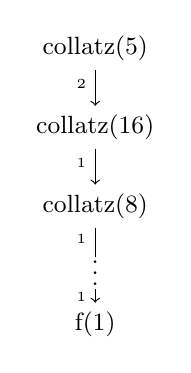
\begin{tikzpicture}\small
% nodes
\node (f1) at (0, 2) {collatz(5)};
\node (f2) at (0, 1) {collatz(16)};
\node (f3) at (0, 0) {collatz(8)};
\node (fn) at (0, -0.75) {$\vdots$};
\node (f0) at (0, -1.5) {f(1)};
% arrows
\draw[->] (f1) --node[pos=0.4, left, label distance=5mm]{\tiny{2}} (f2);
\draw[->] (f2) --node[pos=0.4, left, label distance=5mm]{\tiny{1}} (f3);
\draw (f3) --node[pos=0.4, left, label distance=5mm]{\tiny{1}} +(0, -0.65);
\draw[<-] (f0) --node[pos=0.4, left, label distance=5mm]{\tiny{1}} +(0, 0.45);
\end{tikzpicture}
  \vspace{-10pt}
  \caption{Callgraph of \texttt{collatz(5)}}
  \label{tr_callgraph}
\end{wrapfigure}

Single recursive functions are a subgroup of general recursive functions. They have a linear branching behaviour (\autoref{tr_callgraph}). The function as a whole may contain multiple callsites anyway, as long as each evaluation scenario contains only a single callsite. This is also the only criterion to detect single recursive functions.

The function that computed the length of the \textit{collatz-series} (\autoref{lst:collatz_udf}) is an example for a single recursive function.

\begin{figure}[h]
    \centering
    \begin{minipage}[b]{.45\linewidth}
    \centering
    \sqlcode{snippets/collatz.sql}
    \subcaption{UDf computing the length of the \textit{collatz-series} for a start number $\texttt{n} > 0$.}
    \label{lst:collatz_udf}
    \end{minipage}
    \begin{minipage}[b]{.5\linewidth}
    \centering\scriptsize
        \begin{tabular}{|p{1em}|p{3.3cm}|p{2.9cm}|}\hline
        \cellcolor{gray!25} & \texttt{\phantom{NOT }n=1} & \texttt{1}\\\hline
        \end{tabular}
        
        \begin{tabular}{|p{1em}|p{3.3cm}|p{2.9cm}|}\hline
        \cellcolor{gray!25} $\ast$ & \texttt{NOT n=1 AND \phantom{NOT }n \% 2 = 0} & \texttt{1 + collatz(n / 2)}\\\hline
        \end{tabular}
        
        \begin{tabular}{|p{1em}|p{3.3cm}|p{2.9cm}|}\hline
        \cellcolor{gray!25} $\ast$ & \texttt{NOT n=1 AND NOT n \% 2 = 0} & \texttt{1 + collatz(3 * n + 1)}\\\hline
        \end{tabular}
        \vspace{2em}
    \subcaption{Scenarios of \texttt{collatz}. Each recursive scenario contains just a single callsite.}\label{collatz_scenarios}
    \end{minipage}
    \caption{}
    \label{collatz_sql_with_scenarios}
\end{figure}

The evaluation happens thus also in a strict linear manner. As each scenario depends only on the result of the previous result, the work-around (see \autoref{macro:evaluation_cte}) to access all previous computed results becomes unnecessary. In each iteration exactly one result is computed and in the next iteration the dependant scenario will be evaluated. No need to add all previous results to the current result to have those rows available later (\autoref{opt_sr_evaluation_cte}). Only actually new rows are added to the results.

\begin{figure}[h!]
    \centering
    \begin{minted}{postgresql}
WITH RECRUSIVE
    ...
    evaluation(in_1, res) AS (
        (TABLE basecases)
        
        UNION ( -- was UNION ALL
            WITH e AS (TABLE evaluation)
            (<eval_recursive_scenario_sr(scenario[1])>)
               UNION ALL
            (<eval_recursive_scenario_sr(scenario[2])>)
        )
    )
SELECT ...
    \end{minted}
    \caption{Simplified evaluation-template for single recursive UDFs.}
    \label{opt_sr_evaluation_cte}
\end{figure}

Furthermore, the rather complicated relational division, pivoting and filtering for evaluable scenarios (\autoref{macro:recursive_scenario_evaluation}) can be replaced by a much simpler query (\autoref{opt_sr_eval_scenario}). Because each scenario has only a single callsite, no grouping/partitioning is required to collect results of dependant callsites and to check whether all dependencies are available. If a result of the callsite is present, the scenario can be evaluated. What remains is basically a simple join (\autoref{opt_sr}).

\begin{figure}[h!]
    \centering
    \sqlcode{snippets/opt_sr.sql}
    \caption{Simplified template for single recursive UDFs. Note how the \texttt{FROM}-clause is just a simple join and no \texttt{WHERE} is required anymore.}
    \label{opt_sr_eval_scenario}
\end{figure}



\section{Tail Recursion}

\begin{wrapfigure}{r}{0.5\textwidth}
  \vspace{-10pt}
    \sqlcode{snippets/collatz_tr.sql}
  \caption{Tail recursive formulation of \texttt{collatz}}
  \label{lst:fib_tr}
\end{wrapfigure}

A special form of single recursive functions are tail recursive functions. They do not have any evaluation context around any callsite so that each recursive scenario just returns another recursive call. Eventually, the result of the basecase is just passed all the way up in the callgraph to the root without any modifications. This last phase can therefore be skipped, which means that no \texttt{evaluation}-CTE is required.

The final result is present in the \texttt{basecase}-CTE. The basecase-CTE contains only a single value because single recursive functions have no branches in the callgraph (cp. \autoref{tr_callgraph}). The modifications on the template amount to removing the \texttt{evaluation}-CTE and changing result selection as shown in \autoref{tr_opt_template}. Furthermore the \texttt{callsite\_id}-column can be removed from the \texttt{callgraph}-CTE because the only use of the \texttt{callsite\_id} is to identify the corresponding scenario during evaluation, which is now omitted (\autoref{marco:collect_call_maybe_optimized}).

\begin{figure}
    \centering
    \sqlcode{snippets/opt_tr.sql}
    \caption{Template for tail recursive UDFs. No \texttt{evaluation}-CTE is required anymore as all the basecases already return the final result.}
    \label{tr_opt_template}
\end{figure}


\begin{figure}[h!]\centering\small
    \begin{minted}{postgresql}
    <collect_call_maybe_tr(in_arg_1, predicate, callsite)>
        := SELECT
             in_arg_1                    AS in_1, 
           --callsite.id                 AS callsite_id,
             callsite.arg_1[in_arg_1/$1] AS out_1
           FROM predicate AS p(is_true)
           WHERE p.is_true
    \end{minted}
  \caption{Pseudocode to generate a single call to the callstack-table, optimized for tail recursive UDFs. The callsite id is no longer required as the evaluation-phase is skipped.}
  \label{marco:collect_call_maybe_optimized}
\end{figure}

To test whether an UDF is tail recursive, all its scenarios must be tail recursive. This means that the context of the only callsite \texttt{f(...} must be present at the top level of the query or nested in trivial \texttt{SELECT}s. Any computations like \texttt{1+(SELECT f(n))} would create a computation context around the call that need to be evaluated.

\begin{figure}
    \centering
\begin{minted}{postgresql}
q := f(...)
q := (SELECT <q>)
q := (WITH [<alias> AS (<nonrecursive sql>), ...] <q>)
\end{minted}
    \caption{Grammar for tail-recursive queries. This notion could be extended, but catches most cases as it is.}
    \label{tr_grammar}
\end{figure}

CTEs can be included in the query, if they are only referenced from the callsite-arguments. Callsite-arguments are evaluated during callgraph creation. During evaluation, the callsites including their arguments are replaced by references to their results. So, CTEs are present but unused during evaluation. The resulting query is therefore eligible for the tail recursive optimization.

\section{Constant argument removal}

Some functions have arguments that are always just passed on to subsequent calls without modification, eg. configuration parameters. As these parameters do not change, it is not necessary to include them in the callgraph-table or to include them when matching rows by arguments. The argument can just be left as it is in the translation, eg. as \texttt{\$1}.

\begin{wrapfigure}{r}{0.66\textwidth}
  \vspace{-10pt}
    \sqlcode{snippets/sieve.sql}
  \caption{Sieve of Eratosthenes. \texttt{sieve(2, ARRAY[1, 2, 3, ..., n])} computes all prime numbers up to \texttt{n}.}
  \label{lst:sieve_udf}
\end{wrapfigure}

Omitting unnecessary arguments saves memory as well as CPU-time. The two tables \texttt{callgraph} and \texttt{evaluation} are joined in each iteration of the \texttt{evaluation}-CTE by the function arguments. Removing unnecessary comparisons speeds up the query and saves memory as the same value is not copied again and again.

No change to the template is necessary and detection of constant arguments is straight-forward: The nth argument of a UDF is constant if the nth argument in each callsite is just \texttt{\$n}. The argument is just removed from the list of arguments so that the argument is not considered when filling out templates.

\begin{figure}[h]
    \centering\footnotesize
    \begin{minipage}[b]{\linewidth}
    \centering
    \begin{tabular}{c|c|c|c|c}
         in\_1 & in\_2                                     & callsite\_id & out\_1 & out\_2                                  \\\hline
         2     & \mintinline{postgresql}{ARRAY[2, 3, ..., 7]} & 1            & 3      & \mintinline{postgresql}{ARRAY[2, 3, ..., 7]}\\
         3     & \mintinline{postgresql}{ARRAY[2, 3, ..., 7]} & 1            & 4      & \mintinline{postgresql}{ARRAY[2, 3, ..., 7]}\\
    \end{tabular}
    \subcaption{\texttt{callgraph}-CTE for \texttt{sieve} without optimization}
    \label{}
    \end{minipage}\par
    \vspace*{15mm}
    \begin{minipage}[b]{\linewidth}
    \centering
    \begin{tabular}{c|c|c}
         in\_1 & in\_2                                     & result                                  \\\hline
         4     & \mintinline{postgresql}{ARRAY[2, 3, ..., 7]} & \mintinline{postgresql}{ARRAY[2, 3, 4, 5, 6, 7]}\\
         3     & \mintinline{postgresql}{ARRAY[2, 3, ..., 7]} & \mintinline{postgresql}{ARRAY[2, 3, 4, 5, 7]}\\
         2     & \mintinline{postgresql}{ARRAY[2, 3, ..., 7]} & \mintinline{postgresql}{ARRAY[2, 3, 5, 7]}\\
    \end{tabular}
    \subcaption{\texttt{evaluation}-CTE for \texttt{sieve} without optimization}
    \label{}
    \end{minipage}
    \caption{}
    \label{}
\end{figure}

\begin{figure}[h]
    \centering
    \begin{minted}{postgresql}
SELECT c.in_1                                  AS in_1, 
       (SELECT array_agg(T.v)
        FROM unnest($2) AS T(v)
        WHERE (T.v = c.in_1 OR T.v % c.in_1 <> 0)
          AND T.v = ANY((SELECT e.result)))       AS result
FROM calls_to_basecases c
WHERE (SELECT (2 * c.out_1) > (array_length($2, 1))
    \end{minted}
    \caption{Evaluation of a nonrecursive scenario of \texttt{sieve} inside the \texttt{basecases}-CTE with constant argument removal. Note that \texttt{\$2} is not replaced by \texttt{c.in\_2}.}
    \label{fig:my_label}
\end{figure}

\section{Handling unhashable types}

In some places within the templates we use the duplicate eliminating \texttt{UNION} which internally depends on the "equals" member of its B-tree operator class \cite[p. 1042 f.]{psql}. Equality can be determined either by sorting, which is used as first choice, or by hashing. Custom types uses the sorting operator of its components but lack a default hashing operator.

An undocumented quirk of PostgreSQL is that \texttt{UNION} within \texttt{WITH RECURSIVE} can just use hashing for duplicate elimination\footnote{see \url{https://www.postgresql-archive.org/Hashable-custom-types-td5801576.html}, last accessed at 29/12/2018}. Therefore an error \textit{all column datatype must be hashable} is thrown. This is undesireable, because our goal is that the translation should behave exactly like the original and raise no unexpected errors.

A workaround is to cast unhashable types to \texttt{TEXT} when saving in a table and casting it back to the original type whenever using it. Unhashable types can occur in the arguments and in the return type.

If the return type is not hashable, the result from each evaluated scenario must be casted to \texttt{TEXT} before storing into \texttt{basecases} resp. \texttt{evaluation}. When replacing the result of a callsite with an reference to \texttt{evaluation}, it must be casted back to the original type. Within the final result selection the result must be also casted back to the original type.

Hashable arguments must be casted to \texttt{TEXT} when creating the \texttt{callgraph}. To evaluate the callsite-arguments, the reference to the \texttt{out}-columns must be casted back to the original type. The same is required when replacing arguments during scenario-evaluation.

Unhashable types are detected by introspecting PostgreSQL (\autoref{sql:hashable_query}). This makes the translation aware of custom hash-operators. PostgreSQL has some type-aliases defined, eg. \texttt{smallint} is an alias for \texttt{int2}. The first is returned by \texttt{t.oid :: regtype} and the latter by \textit{t.typename}.

\begin{figure}
    \centering
\begin{minted}{postgresql}
SELECT t.typname :: TEXT 
FROM pg_operator as o, pg_type as t 
WHERE o.oprleft = t.oid 
  AND o.oprright = t.oid 
  AND o.oprname = '=' 
  AND o.oprcanhash 

UNION

SELECT t.oid :: regtype  :: TEXT 
FROM   pg_operator as o, pg_type as t 
WHERE o.oprleft = t.oid 
  AND o.oprright = t.oid 
  AND o.oprname = '=' 
  AND o.oprcanhash;
\end{minted}
    \caption{Query to obtain all type-aliases from a PostgreSQL-instance that have an operator defined that can be used for hashing.}
    \label{sql:hashable_query}
\end{figure}